\documentclass{article}

\usepackage[tc]{titlepic}
\usepackage{graphicx}
\usepackage{hyperref}
\usepackage[font={small,it}]{caption}
\usepackage{float}
\usepackage{textcomp}
\usepackage{pdfpages}
\usepackage{pdflscape}
\usepackage{listings}
\usepackage{multirow}
\usepackage{longtable}
\usepackage{pifont}

% Include paragraph sections in contents
\setcounter{tocdepth}{4}

\makeatletter
% display heading, like subsubsection
\renewcommand\paragraph{\@startsection{paragraph}{4}{\z@}%
                                     {-3.25ex\@plus -1ex \@minus -.2ex}%
                                     {1.5ex \@plus .2ex}%
                                     {\normalfont\normalsize\bfseries}}
 \setcounter{secnumdepth}{4}
\makeatother

\lstdefinelanguage{JavaScript}{
  keywords={typeof, new, true, false, catch, function, return, null, catch, switch, var, if, in, while, do, else, case, break},
  keywordstyle=\color{blue}\bfseries,
  ndkeywords={class, export, boolean, throw, implements, import, this},
  ndkeywordstyle=\color{darkgray}\bfseries,
  identifierstyle=\color{black},
  sensitive=false,
  comment=[l]{//},
  morecomment=[s]{/*}{*/},
  commentstyle=\color{purple}\ttfamily,
  stringstyle=\color{red}\ttfamily,
  morestring=[b]',
  morestring=[b]"
}

\lstset{
   language=JavaScript,
   extendedchars=true,
   basicstyle=\footnotesize\ttfamily,
   showstringspaces=false,
   showspaces=false,
   numbers=left,
   numberstyle=\footnotesize,
   numbersep=9pt,
   tabsize=2,
   breaklines=true,
   showtabs=false,
   captionpos=b
}

\captionsetup{justification=centering}

\title{%
  DC4400 Project Report \\
  \vspace{0.2cm}
  \small Extension of the BBC iPlayer off product schedules system to process change notifications
}

\titlepic{
\includegraphics[width=0.3\textwidth]{assets/aston.png}}

\author{Oliver Matthew Bowker (220263618)}
\date{\today}

\begin{document}

  \maketitle

  \newpage

  \tableofcontents
  \newpage

  \listoffigures
  \newpage

  \listoftables

  \newpage
  \section{Executive Summary}

\subsubsection*{Problem Statement}
SpaceChimp is a team in the BBC Partnerships group that is responsible for providing schedules data for live programming for all BBC channels to 
external partners. This system was designed to replace an external dependency the BBC had with a data provider. There is currently a system set up 
that statically generates this data every 15 minutes. This can leave to outdated User Interfaces (UIs) for partners as the data can be up to 15 minutes 
out of date, therefore displaying and linking users across the UK to the wrong or unavailable content.

\subsubsection*{Proposed Solution}
The current static system is to be updated to handle delta notifications that enable the updating and deleting of individual schedules instead of a 
refresh of all schedules every 15 minutes. To achieve this upgrade multiple steps must be taken:

\begin{itemize}
  \item An initial design will be created with architecture and algorithm, this design can then be implemented in a software spike to discover 
  problems and solutions.
  \item The work done in the spike will drive the design of the real product. This will be broken down into tasks and feature sets that developers 
  within the team will work on. Research will be done as part of this spike to find alternate routes where needed and will be presented in a spike 
  document.
  \item These tasks will go through the standard procedures of an enterprise team, development, testing and releasing. This development will include 
  handling of delta notifications, a garbage collector and integration and comparison tests to help gain confidence in the new system.
  \item Strategies to release the code into a live environment, used by 10s of millions of peoples, will be discussed and a release strategy for partners 
  will be decided upon.
\end{itemize}

\subsubsection*{Value}
This new system will allow the teams schedule offering to be as up to date as possible. When a partner requests the current data for a schedule to display in 
their UI they will get the most up to date information possible. This work will also open up the possibility to send update notifications directly to partners
so they no longer rely on requesting data at intervals, and can request only the data that has been updated since their last call.

\subsubsection*{Final Thoughts and Next Steps}
This new system will lower overall processing time and cost due to schedules only be updated and deleted when needed. It will help partners offer more up to 
date UIs for their customers, help the BBC reach more people and reduce some overhead from external data providers. There is scope to extend this project 
further in the future to include notifications directly to partners as well as research and designs into how the new single-threaded system could one day 
be parallelised.

\vspace{0.2cm}
\noindent This report and it's content can be found in the following GitHub repo: \href{https://github.com/OMBowkerBBC/DC4400-Report}{DC4400-Report}.

\newpage

  \section{Introduction}

  The BBC is now over 100 years old (BBC, 2022) and is well known for it's TV channels and radio stations that are broadcast over the airwaves (Pilnick, Baer, 1973, p.3) 
  to peoples homes across the UK. However this old way of broadcasting, sending out airwaves on a certain frequency to an antenna, is becoming 
  less popular in the modern age of the internet. A study done by Ofcom showed that people
  \textit{'watched on average about 16\% less broadcast TV between 2019 ... and 2022'}, with viewing \textit{'decreasing by 47\%'} (Ofcom, 2023, p.7) between ages
  16-24. In addition another study carried out by media analyst firm Ampere found that in 2021 37\% of people claimed to watch no linear TV,
  this increased to 45\% by 2023 (Ampere Analysis, 2023).
  
  This fall correlates with the significant rise in internet enabled TVs in the home, with statista finding that 
  \textit{'In 2014 just 11 percent of households in the UK owned a Smart TV, whereas, in 2023, nearly 74 percent of households reported owning a Smart TV.'} (Statista, 2023).

  \begin{figure}[H]
    \centering
    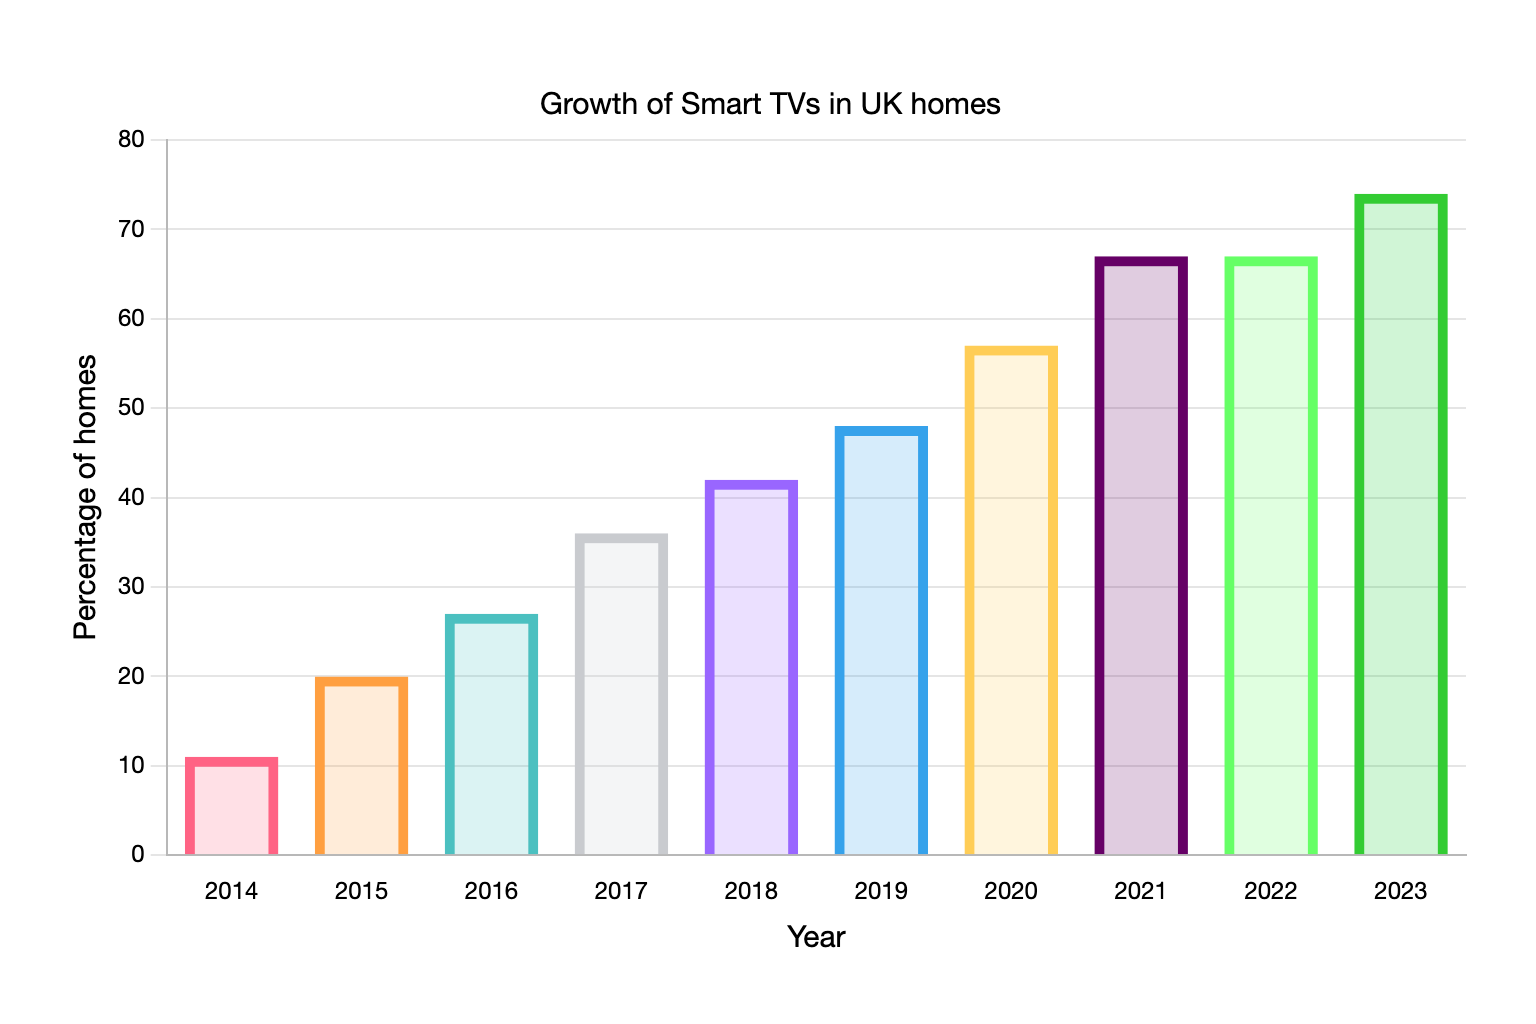
\includegraphics[width=6cm]{assets/smartTvGrowth.png}
    \caption{Bar chart showing growth of smart TVs in UK homes (Statista, 2023) \textit{Created with Line Graph Maker} (Line Graph Maker, 2023)}
    \label{fig:smartTvGrowth}
  \end{figure}

  Some of these devices still support OTA broadcasts, however devices like the Amazon Fire TV stick and Googles Chromecast, are purely internet
  based; However they do offer a \textit{'guide/epg'} section with Amazon having a development guide (Amazon, 2021) on how to integrate with it.
  Director general of the BBC, Tim Davie, in 2022 stated:
    \begin{quote}
      \textit{'The vision is simple: from today we are going to move decisively to  a digital-first BBC'} (Davie, 2022)
    \end{quote}

  This statement highlights the goal to put more organisational focus on these new forms of media and internet enabled devices. 
  
  This report will discuss an upgrade carried out to the BBCs \textit{'off-product'} schedules system, responsible for delivering up to date schedules to
  partners such as Freeview, Amazon and more. First I will give some background on the project, where I will discuss topics including database
  management in parallel/multi-threaded systems, cloud computing and the power of microservices and strategies to protect live code systems in a CI/CD
  environment. I will also give some background on the starting architecture of the system and how the changes align with the BBCs and teams OKRs (Sparks, 2024).
  
  Following that, I will discuss the work that was done. This will be broken down into 5 sections that align with our teams ways of working flow.
  \begin{enumerate}
    \item Requirements and epic creation
    \item Investigation and Spike
    \item Slicing and task/ticket creation
    \item Development of software
    \item Releasing of software
  \end{enumerate}

  I will then talk about the outputs of the project. Theses will include burn-up charts for the projects, dashboards created, documentation of the final 
  architecture and a description of the exact final product.

  Finally I will discuss potential improvements for future iterations. This will range between small code changes to a complete re-architecture of the system.
\newpage

  \section{Background}

\newpage

  \section{Research}
  I will now explore research done relating to the project specified. This will outline some design decisions that were made and link to other 
  sections of the report where they may be explored more. This section will explore parallelism and thread safety focusing on data stores as well as 
  CI/CD, it's pros and cons when deploying to live systems and how we as a team worked around it.

  \subsection{Storage Solutions and Parallelism}
  \label{sec:storageSolutions}

  Currently the schedule pipeline consists of two components, the ingester, followed by the schedule generator. The first part of this pipeline is
  parallelised, multiple lambdas can be run at the same time to insert data into the Redis. This is a harder task for the schedule generator to do,
  as it needs update a list of linked schedules to an episode in the Redis store. This data can be edited through multiple streams, both the schedule
  catalogue pipelines, meaning the array could easily become incorrect/polluted. Sharing memory in a threaded/parallelised system is a well-known 
  challenge and you need to know when it's safe to update/edit this memories value (Grossman, 2023).
  This is also known as being thread safe which can be described as \textit{'different threads can access the same resources without exposing erroneous 
  behaviour or producing unpredictable results'} (Ugarte, 2024).

  \begin{figure}[H]
    \centering
    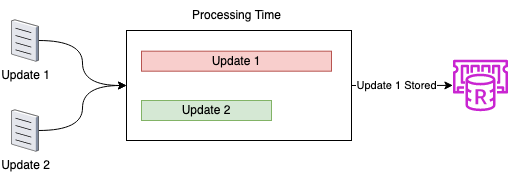
\includegraphics[width=6cm]{assets/raceCondition.drawio.png}
    \caption{Diagram showing how a broadcast list of an episode can become incorrect/polluted.}
    \label{fig:raceCondition}
  \end{figure}

  \subsubsection{Redis and Elasticache}
  We use amazons Elasticache (Amazon Web Services, 2024f) for our Redis (REmote DIctionary Server) solution as it stores data in memory, which makes it 
  quick to retrieve stored data (IBM, 2024). This is vital for us as we store large documents that need to be retrieved and sent to partners on 
  an API request. Redis is single-threaded but supports concurrency, \textit{'when at least two threads are making progress'} (Oracle Corporation, 2010) 
  which is not the same as parallelism, \textit{'when at least two threads are executing simultaneously'} (Oracle Corporation, 2010).

  \begin{figure}[H]
    \centering
    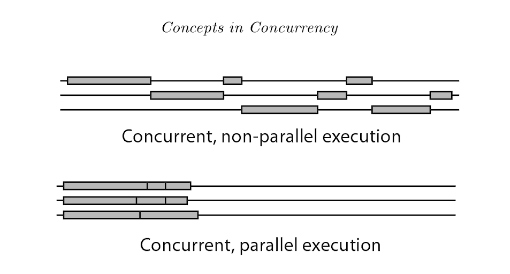
\includegraphics[width=8cm]{assets/concurrecnyVsParallelism.jpg}
    \caption{Difference between concurrency and parallelism (Sottile, Mattson, Rasmussen, 2009, p.25).}
    \label{fig:concurrecnyVsParallelism}
  \end{figure}

  This concurrency allows Redis to support multiple requests at once, but it cannot do multiple operations at once; although more recent versions are allowing
  some safely threaded operations such as deleting records (Redis Ltd, 2024a). It also supports batch uploading and blocking commands. However these also 
  don't help keep the data thread-safe.

  \begin{itemize}
    \item \textbf{Pipelining} - Pipelining sends a block of commands at once however does not guarantee that commands sent are done in sequence 
    (Redis Ltd, 2024b).
    \begin{figure}[H]
      \centering
      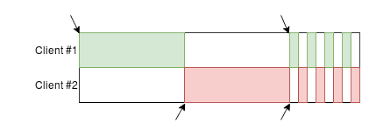
\includegraphics[width=8cm]{assets/pipelineOrdering.png}
      \caption{How Redis pipelines don't guarantee sequential execution (Eyng, 2019).}
      \label{fig:pipelineOrdering}
    \end{figure}
    \item \textbf{Transactions} - Transactions are very similar to pipelines however, guarantee that the transactions commands are not interrupted by another
    clients requests and are therefore executed in sequence (Redis Ltd, 2024c).
    \item \textbf{Blocking Actions} - Blocking actions stop the current client from executing commands until the blocking action is complete. However other 
    clients can still send requests to the server whilst this client is blocked (Redis Ltd, 2024d). 
  \end{itemize}

  The options above still allow the previous race condition to occur, as instances of the schedule generator may vary in processing time and therefore the 
  time of writing to the Redis cannot be guaranteed to be in order of the events.

  \subsubsection{How thread-safety can be achieved}
  When researching and spiking (Visual Paradigm, 2024) the project, other technologies were found that could help offer thread safety whilst parallelising
  the schedule generator. These were types of store/database locking mechanisms.

  \begin{itemize}
    \item \textbf{Pessimistic Locking} - This method \textit{'assumes that access to shared memory will be contended'} (Weston, 2011) and
    acquires a lock on the data to be edited. Any other client/connection attempting to edit this data must wait until this lock is released to update
    the data (Thornton, 2001). This can lead to issues such as deadlock which is when two clients are both awaiting on each other's lock to 
    be released. This can end up with both clients being stuck in an endless cycle of waiting for each other (Thornton, 2001; Apache Software Foundation, 2013).

    \begin{figure}[H]
      \centering
      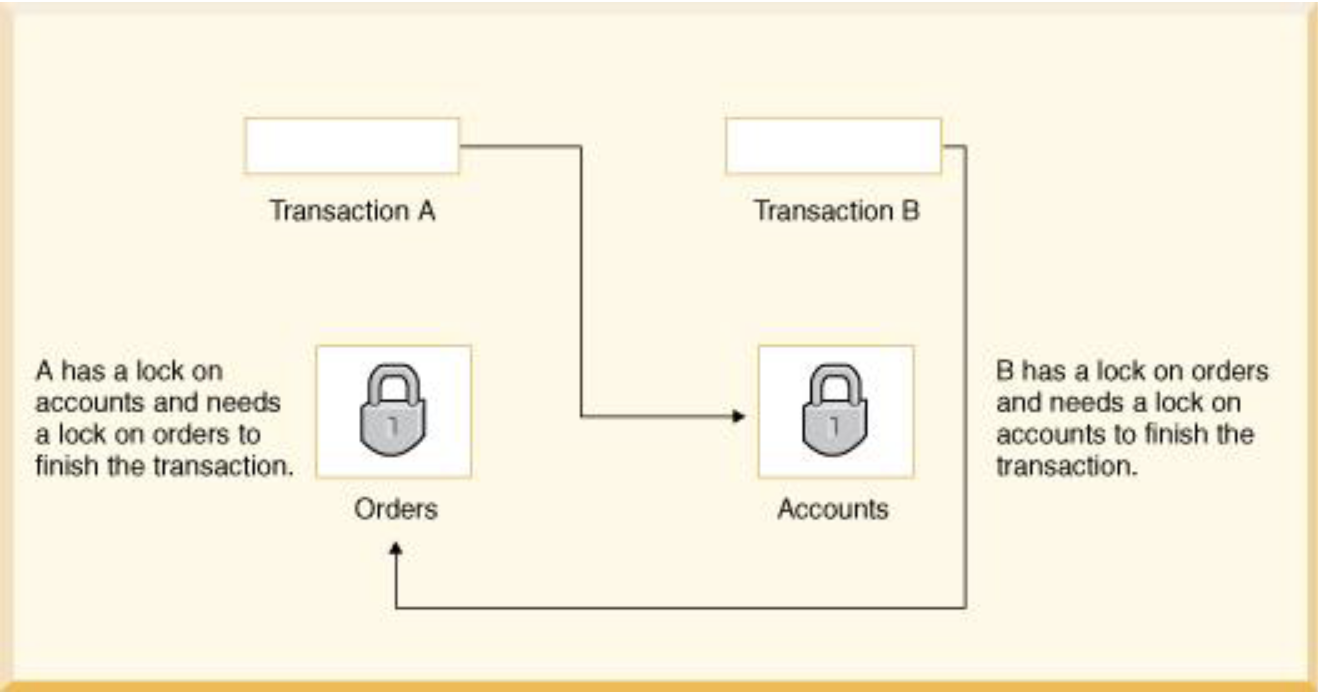
\includegraphics[width=8cm]{assets/deadlock.png}
      \caption{Example of a deadlock scenario (Apache Software Foundation, 2013).}
      \label{fig:deadlock}
    \end{figure}

    There is also a situation where a client locks a piece of data and for one reason or another halts, this would cause needless delay, when a timeout is 
    specified, if a timeout is not specified then this object would be locked from changes indefinitely (Thornton, 2001).

    \item \textbf{Optimistic Locking} - This method \textit{'relies on end-of-transaction validation'} (Graefe, 2016) and takes the outlook of presuming
    it's safe to write until the very end (Kanungo, Morena, 2023). Unlike its counterpart (pessimistic locking) it does not lock the record that is 
    being updated. Instead before the new data is written, the original data is checked against the current data stored (Thornton, 2001). If this data doesn't
    match, then a change has occurred during processing and the new data to be written must be re-calculated with the new changes.

    \begin{figure}[H]
      \centering
      \includegraphics[width=6cm]{diagrams/sequence/Optimistic Locking.png}
      \includegraphics[width=6cm, height=6cm]{diagrams/activity/Optimistic Locking.png}
      \caption{Sequence and activity diagrams outlining logic of optimistic locking.}
      \label{fig:optimisticLocking}
    \end{figure}

    This above logic could be implemented into our Redis solution. It would require either a total comparison of the object or a simple \textit{version}
    field that specifies when the object has changed.
  \end{itemize}

  During this investigation DynamoDB (Amazon Web Services, 2024e) was highlighted as a potential option due to it supporting optimistic
  locking. The final decision was to not use it however and stick with the current solution as there was a want to get the project started to keep 
  up with our roadmap and not further investigate this option. There were also more unknowns with this technology as we had never used it before.
  I will discuss a solution using DynamoDB in the \hyperref[sec:future]{\textbf{Future Work}} section of this report.
   
  \newpage
  \subsection{Agile and CI/CD}
  \label{sec:cicd}

  As a team we follow an agile approach to software development, more accurately we follow a Kanban approach. The Kanban methodology 
  \textit{'focuses more on monitoring and improving workflows'} (Heil, C, 2022) and doesn't use concepts such as sprints from scrum (Rehkopf, 2024). 
  Instead, software created using the Kanban approach is deployed/released when it's done (Rehkopf, 2024) and uses a Kanban board where tickets move 
  across columns depicting where they are currently at in development cycle (Mauvius Group Inc, 2021).

  \begin{figure}[H]
    \centering
    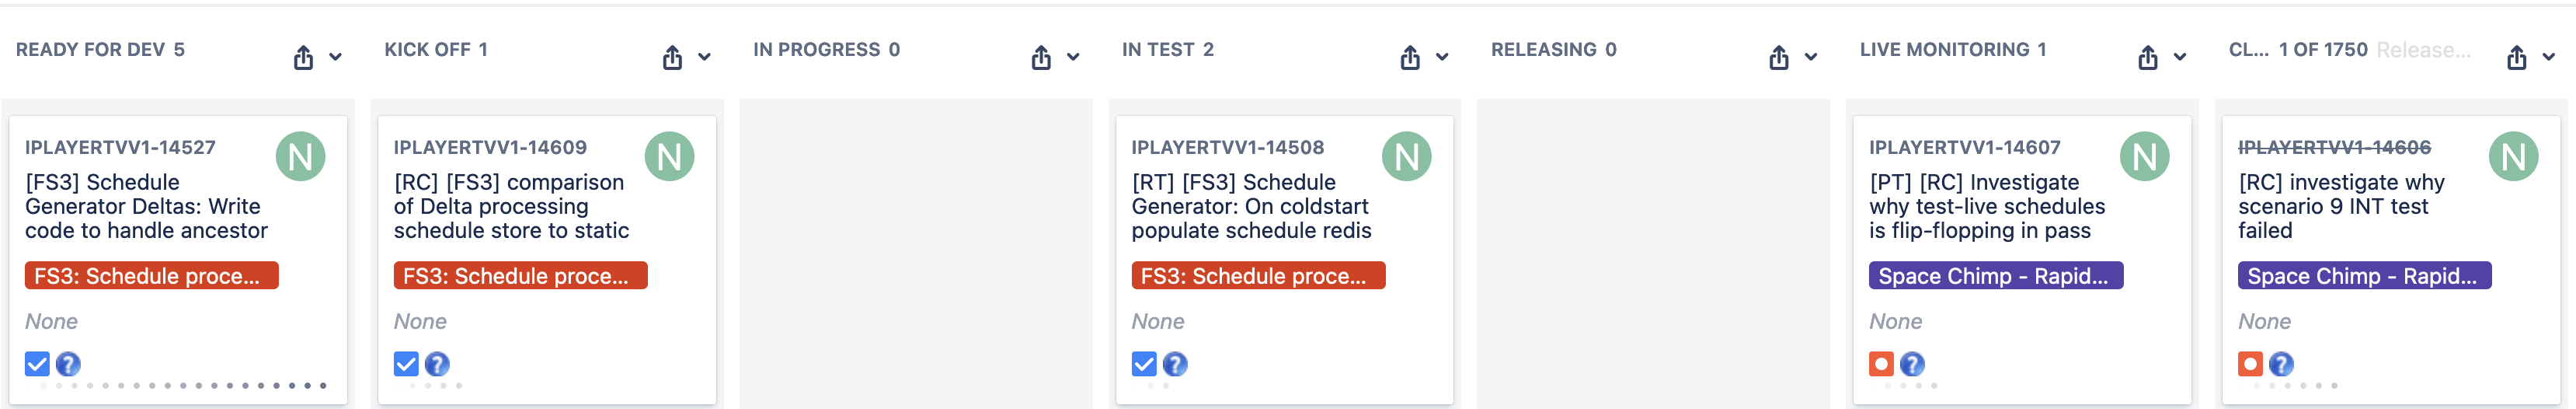
\includegraphics[width=10cm]{assets/kanbanBoard.png}
    \caption{SpaceChimps Kanban board.}
    \label{fig:kanbanBoard}
  \end{figure}

  This workflow fits in well with Continuous Integrations and Continuous Deployment (CI/CD). As a team we release/build all our own code to 
  multiple environments using Jenkins declarative pipelines (Jenkins, 2024).

  \begin{figure}[H]
    \centering
    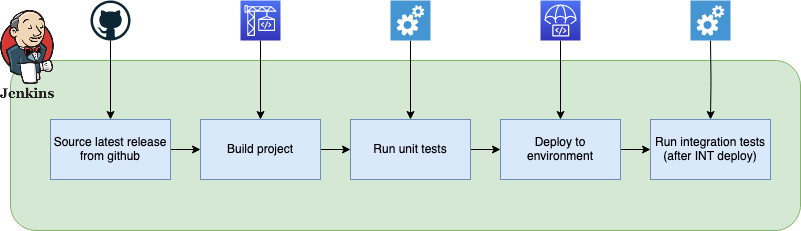
\includegraphics[width=10cm]{assets/pipeline.drawio.png}
    \caption{General pipeline flow.}
    \label{fig:pipeline}
  \end{figure}

  Having these well-defined deployment pipelines makes deploying new code easy and helps manage deployments across multiple environments as configuration 
  can be built into the pipeline (Rodriguez, et al, 2016). This approach allows bugs to be caught faster than when using 
  a \textit{'big bang'} approach, as the bug is likely to be with a single new change (Department of Defence, 2021).
  The additional testing also gives more confidence in the code deployed and rollbacks are made extremely simple due to version control management.

  \vspace{0.2cm}

  There are of course some downsides to CI/CD, whenever an external platform, Jenkins in our case, is being used this opens a new attack vector (NSA, 2023).
  OWASP keeps a list of some of these threats (OWASP Foundation, 2023), however they mostly comprise of poor 
  authentication to CI/CD systems and attacks by people who already have access to source code and the CI/CD platform itself (employees).

  Other issues include maintenance of the pipeline's code/infrastructure and potential complexity (Wikström, 2019),
  this can be especially true when pipelines call other processes. 

  Code quality can become an issue, with technical debt increasing due to the encouraged continuous deployment of new software (Rodriguez, et al, 2016) 
  and more bugs also appear to occur. One study showed that the number of bugs increased when using CI/CD (Fairbanks, Tharigonda, Eisty, 2023).

  \begin{table}[H]
    \centering
    \begin{tabular}{|p{0.3\textwidth}|p{0.15\textwidth}|p{0.15\textwidth}|}
      \hline
      & CI/CD & No CI/CD \\ \hline
      GitHub average issues & 135.38 & 57.33 \\ \hline
      Gitlab average issues & 52.04 & 17.68 \\ \hline
    \end{tabular}
    \caption{Table from study showing difference in issues found between approaches (Fairbanks, Tharigonda, Eisty, 2023).}
  \end{table}
  
  However, this same study also showed a commit velocity increase of 141\%, so it could be argued that these bugs are quickly remedied due to this quicker 
  release time. In addition to this as a team we do pull requests, another developer checks new code before release, which should also mitigate some 
  of the outlined issues above.

  \newpage
  \subsubsection{Software Changeover Strategies}
  The system that is being upgraded is in LIVE use by partners, but the work itself will take time to implement. We don't want to make changes to how
  the LIVE system works for partners, but we do want to test that the new software works on the LIVE environment without a \textit{big bang} deployment.

  There are three main types of changeover strategy, direct (big-bang), parallel running or a phased strategy and its multiple variants (Banerjee, 2017). 
  
  \begin{figure}[H]
    \centering
    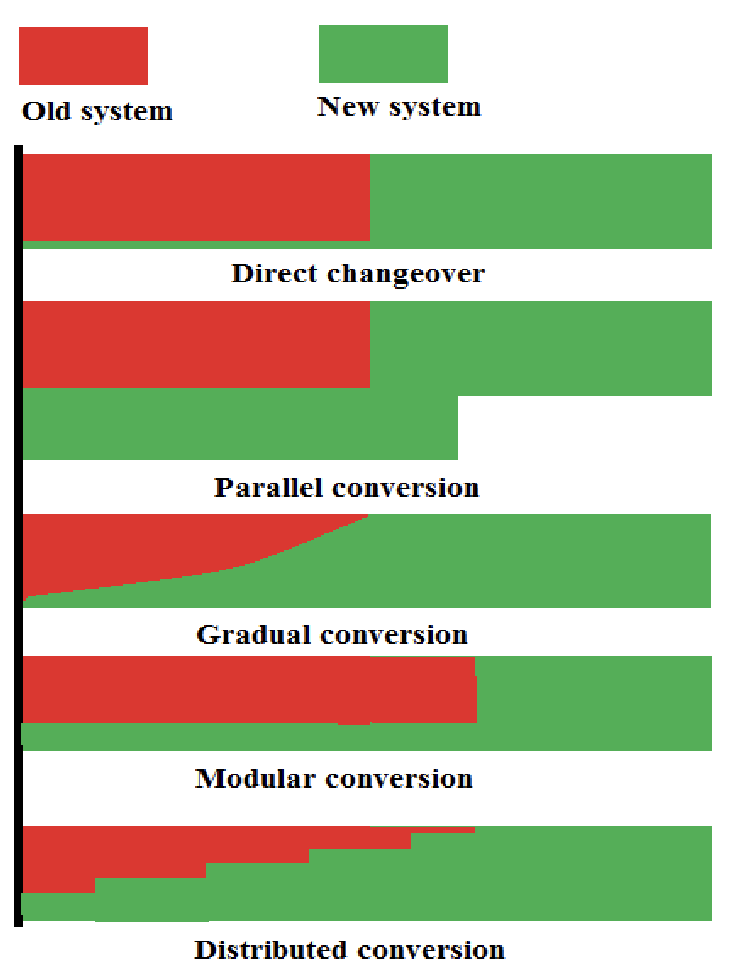
\includegraphics[width=6cm]{assets/changeoverStrategies.png}
    \caption{Timeline of different changeover strategies (Banerjee, 2017).}
    \label{fig:changeoverStrategies}
  \end{figure}
  
  As discussed, a direct approach is risky and could easily run into errors, a phased approach in this situation is also not valuable as the we want 
  to remain consistent in the data we provide to all our partners, so a parallel system is our best option. Temporarily the old and new system will 
  run side-by-side, this will allow us to write comparison tests between the old output and the new (Smyth, 2020).

  In addition to having both systems the data on Redis also needs to be separate as they may differ during development. This will be achieved by 
  using different Redis keyspace prefixes (IoRedis, 2024) to keep the data separate and allow a test to check both for differences (Rustagi, 2023). 
  The partners would continue to get data from the old keyspace, when we are happy with our comparison tests the partners can be swapped over to the new 
  keyspace and the old data can be deleted. 

\newpage
  \section{Work Done}
  In this next section I will discuss the work that was carried on the project. In our team we have \textit{'ways of working'}
  flowchart that helps guides us in how the project should be done throughout the team (GoRetro, 2023). Our ways of working is broken down into 5 sections, 
  all of which will be discussed. For a full diagram of our workflow see \hyperref[sec:AppendixD]{\textbf{Appendix D}}.

  \subsection{Requirements and epic creation}
  The First stage is initiation, what's the project going to be about, how it fits into the companies strategy and OKRs, requirement gathering 
  and epic creation, an epic being a set of user stories/features (Karolis, Saulius, 2023).

  \begin{figure}[H]
    \centering
    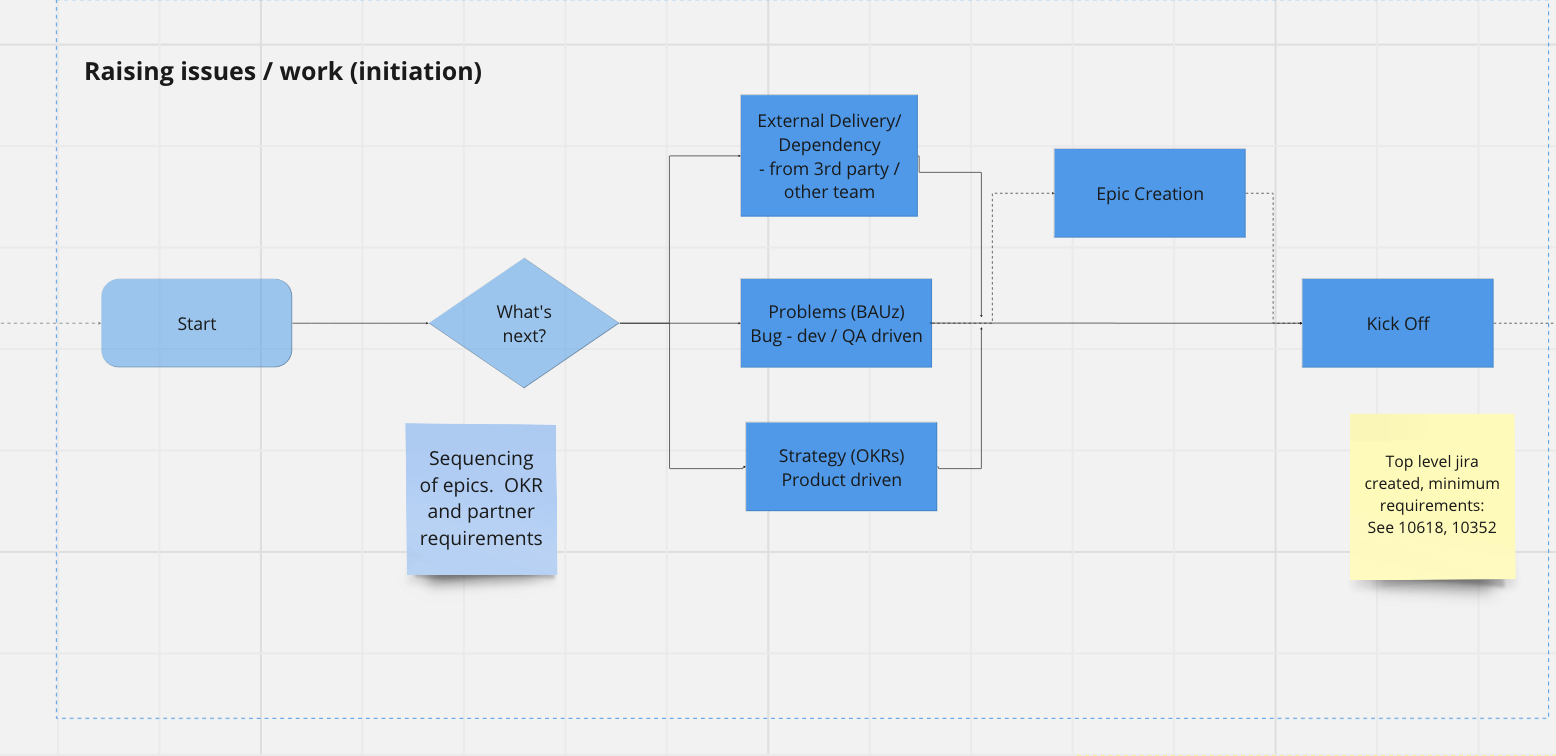
\includegraphics[width=8cm]{assets/workflow/initiate.png}
    \caption{Initiation stage of our ways of working.}
    \label{fig:workflowInitiate}
  \end{figure}

  Due to complications in project allocation, I was not involved in the initial phases of development for this project. However discussions with 
  people that were, highlighted that due to the lack of external partner interaction their wasn't much to discuss and no solid requirements were 
  outlined, only the goal which is to allow the schedule generator to be moved from a static refresh of schedules to an event driven process.

  The benefits of the project and how it achieves our OKRs has been discussed previously in the report. However I want to create some tangible
  requirements here using the MoSCoW framework which consists of must, should, could and won't haves (Eduardo, 2022). I will focus on software
  requirements and denote whether they are functional (F) or non-functional (NF) (Bigelow 2020).

  \begin{enumerate}
    \item (F) The software \textbf{Must} be able to process schedule updates. 
    \item (F) The software \textbf{Must} be able to process episode updates.
    \item (F) The software \textbf{Must} be able to process ancestor updates.
    \item (NF) The software \textbf{Must} keep stored data more relevant than the static version.
    \item (F) The software \textbf{Must} still support a coldstart option.
    \item (F) The software \textbf{Must} contain alarms to alert us to errors.
    \item (F) The software \textbf{Should} gather metrics on processing time and types of updates.
    \item (F) The software \textbf{Should} clean up unneeded data from it's store.
    \item (NF) The software \textbf{Could} support parallelised processing.
  \end{enumerate}

  In this case requirement gathering was easy as there were no partners to discuss the changes with as it's all internal and the output to partners
  stays the same. If this wasn't the case then requirements would have to be gathered from all partners affected or interested in the projects 
  outcome. These requirements would be gathered through meetings and conversations with these partners individually and compromises may have to 
  be made by both sides.
  This is usually the case when there is a requirement conflict, which can be described as:
  \begin{quote}
    \textit{'Requirements conflict is defined as unexpected or contradictory interaction between requirements that has a negative 
    effect on the results (Cameron, Velthuijsen, cited in Kim et al, 2007)'}
  \end{quote}
  These conflicts need to be managed well, as Kim et al (2007) warns these conflicts can \textit{'lead 
  to negative or undesired operation of the system'}. However certain stakeholders will often carry more leverage than another, taking into 
  consideration the Pareto Principle (Sanders, 1987), the 80-20 rule, it's easy for an organisation to leave out requirements of smaller stakeholders.
  A balance must be struck here where all parties are kept happy, without damaging the original idea of the project when large stakeholders try 
  and morph it into what they deem it should be.

  In this case no conflicts occurred due to the how internalised the project is. An epic was created in Jira and theses requirements could then be explored 
  and implemented in the next phase.

  \newpage
  \subsection{Investigation and spike}
  After initiation the project is investigated and then \textit{spiked}. In this case investigation/research for the most part has been done,
  as we knew the system was feasible due to following the same design as our catalogue pipeline. However it was determined that a spike of the 
  proposed algorithm would be done.

  \begin{figure}[H]
    \centering
    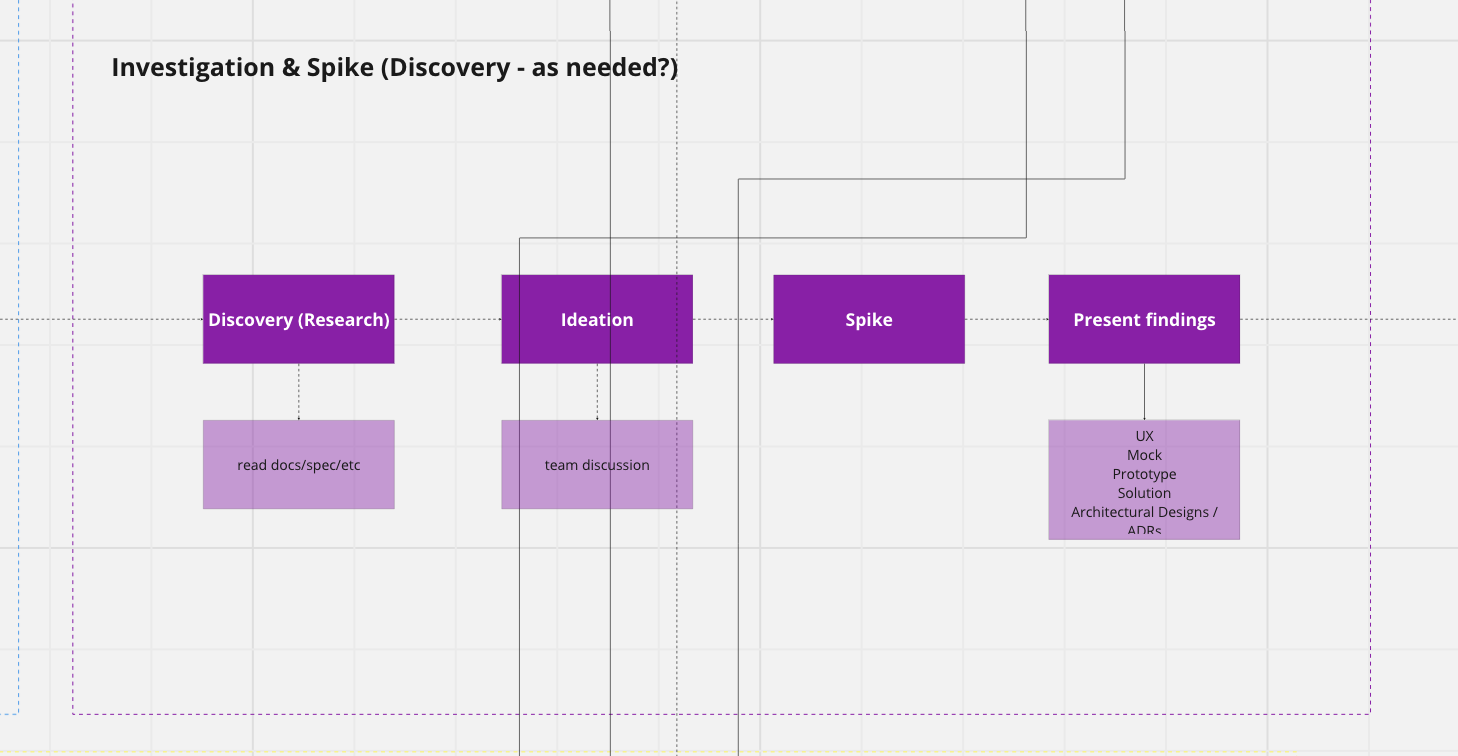
\includegraphics[width=8cm]{assets/workflow/investigation.png}
    \caption{Investigation stage of our ways of working.}
    \label{fig:workflowInvestigation}
  \end{figure}
  
  A spike is often used when there are unknowns about a  project (Visual Paradigm, 2024). A study done by 
  Hashimi and Gravell (2020) found that a majority of people in industry saw spikes as an effective tool and helped in managing risks. In another
  study they also stated that one of key purposes of a spike was to help guide story/ticket estimations (Hashimi, Gravell, 2019). 
  
  In the first paper it was also hypothesised that technical debt can also be lowered through the use of spikes, with technical debt be defined as:
  \begin{quote}
    \textit{'the idea that developers sometimes accept
    compromises in a system in one dimension (e.g., modularity) to meet an
    urgent demand in some other dimension (e.g., a deadline)' (Kruchten et al, 2012)}
  \end{quote}

  Spikes were used by Glas and Hedén (2021) to help bring down technical debt in their study. However when thought about simply, 
  a spike could be seen as a tool to spot the technical debt before it touches live systems. Due to a prototype being made flaws can be spotted 
  early and ironed out before the \textit{'real'} development work begins.

  For the project a spike was carried out to test the algorithms outlined in \hyperref[sec:AppendixC]{\textbf{Appendix C}} to test the 
  throughput of the system and see if it could handle the incoming requests. We used the technical spike template recommended by Microsoft (2021), to 
  document findings and outline the spikes objectives. Hashimi, Abduldaem and Gravell (2022) found that  \textit{'timeboxing, objectives,
  documentation, and clear communication'} were the key factors that lead to a successful spike.

  There was no time limit set, which did lead to scope creep (Martins, 2023) and more time being spent than was necessary. It's important to remember that a 
  spike is not meant to be the final product, however scope creep lead to the spike being almost a fully working system, albeit unrefined and with issues. 
  This is something as a team we have now changed in our process and will always timebox spikes in the future to prevent this.

  Despite this the other key factors were well adhered to. Objectives and documentation of the spike were put into a spike document
  and we had communication with a more senior member of the team at all times as well as daily stand ups to communicate issues/progress on the spike. 
  The full spike document can be seen in \hyperref[sec:AppendixE]{\textbf{Appendix E}}, below are the key findings.

  \begin{enumerate}
    \item A garbage collector should be used to clean up data that is no longer referenced by a schedule. This will help lower the amount of redis sets/gets
    and has no negative affect on partners.
    \item When a catalogue item (episode/series/brand) updates it will also need to update it's associated schedules, for titling and descriptions. This in 
    itself is not a problem, however if the number of schedules referenced is large it can significantly slow the system down. Parallelisation should be 
    looked into, at least at the schedule level to help ease this. Full parallelisation would require a new design to support parallelised editing of the 
    broadcast list held in episodes (this discussed in the \hyperref[sec:storageSolutions]{\textbf{Research}} section).
    \item Redis duplication is complex and is only needed so that episodes can reference a list of schedules that they are in. Might be worth using 
    DynamoDB here as this will also help with parallelisation (This is explored in the \hyperref[sec:future]{\textbf{Future Work}} section).
    \item Additional filtering from the catalogue pipeline could be added to only send updates for items that are referenced by a schedule. This would 
    stop lambda being ran that essentially do nothing, this is also discussed in \hyperref[sec:future]{\textbf{Future Work}}.
  \end{enumerate}

  It was determined by the team that, for now, the system should be single-threaded and stick to the original design due to time constraints.
  Parallelisation could be looked into in the future when we had some time. However it was agreed for a garbage collector to be used and 
  when a batch of schedule updates is is triggered by a catalogue update that some form of concurrency would be required. This can be done with schedule
  objects due to the single threaded nature of the current system. As the schedule updates are being done because of a catalogue update the only 
  fields that can change are the titles and descriptions. These do not affect or reference anything other than the object itself.

  \begin{figure}[H]
    \centering
    \includegraphics[width=8cm]{diagrams/activity/Schedule Concurrency.png}
    \caption{Simple activity diagram showing basic concurrency logic for updating schedules triggered by a catalogue update.}
    \label{fig:scheduleConcurrency}
  \end{figure}

  \newpage
  \subsection{Slicing and kick-off}
  Another small section is the \textit{'kick-off'}, usually a single meeting where the team gets together and discusses the tickets that makeup
  the project as a whole. 

  \begin{figure}[H]
    \centering
    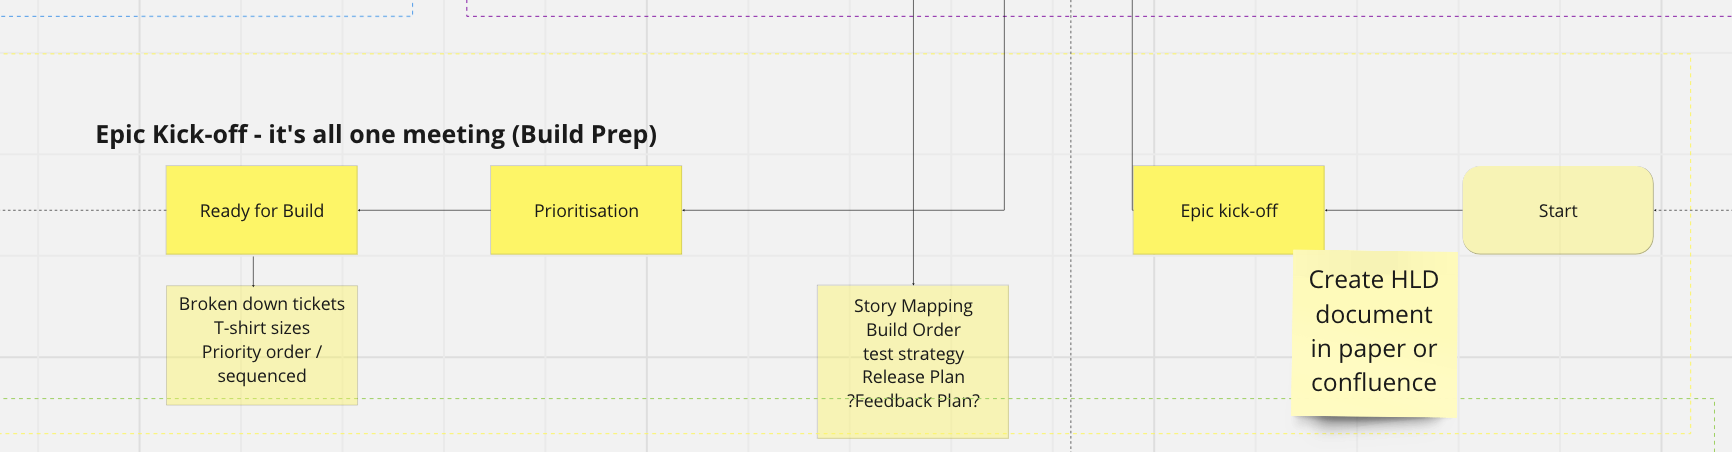
\includegraphics[width=8cm]{assets/workflow/kickoff.png}
    \caption{Kick-off stage of our ways of working.}
    \label{fig:workflowKickOff}
  \end{figure}
  
  Ideally this work has already been broken down into tasks. This is where the spike really helps, instead of guessing we are able to better understand 
  the work that needs doing and create tasks accordingly (Hashimi, Abduldaem, Gravell, 2022). The following diagram shows the initial breakdown of 
  tasks/tickets that were created for the project.

  \begin{figure}[H]
    \centering
    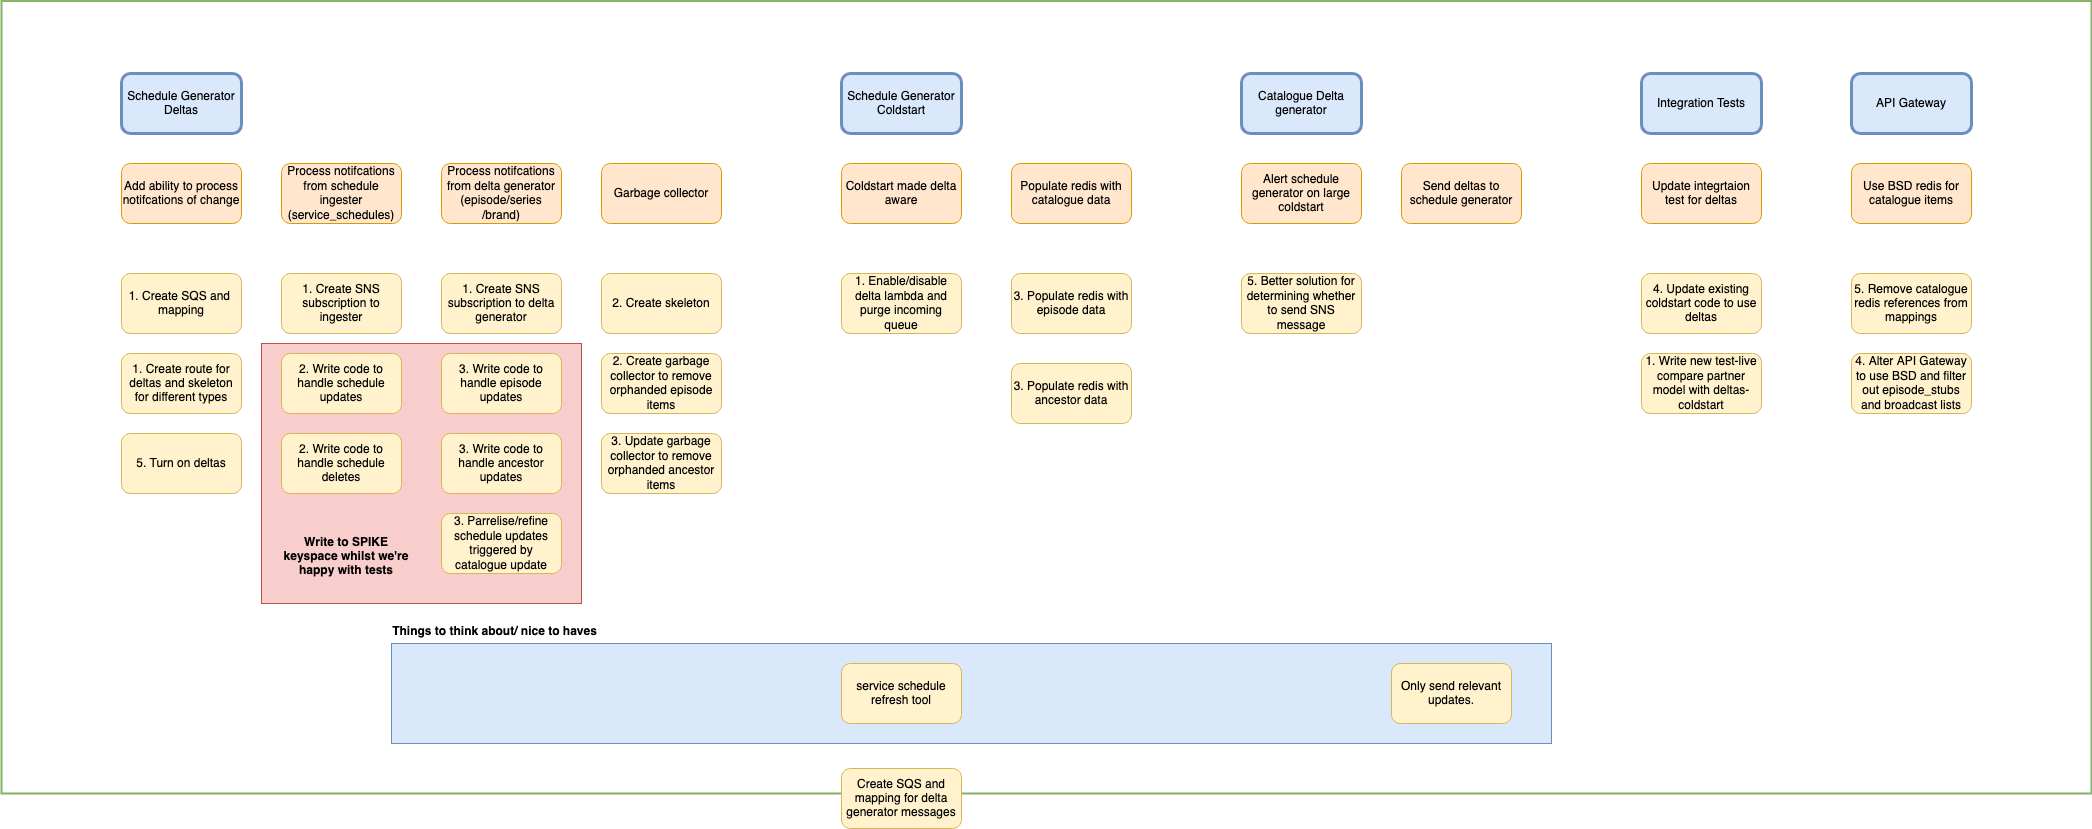
\includegraphics[width=14cm]{assets/schedulesSlicing.drawio.png}
    \caption{Pre-work slicing of work, organised vertically into components.}
    \label{fig:schedulesSlicing}
  \end{figure}

  A work breakdown structure (WBS) is a tool used to \textit{'break down deliverables into sub-deliverables to visualize projects'} (Raeburn, 2024) 
  and is typically broken down into 3 levels, parents, dependencies and sub-tasks, however it can consist of as any as a team wants. For the above I kept it 
  at 3 levels, going vertically, blue represents self-contained features/components, orange is a parent task to complete the feature and yellow is a 
  sub-task of the parent task. Numbers on the sub-tasks represent the initial prioritisation/ordering of the tasks into slices or feature sets.
  
  It's important to note that this is not the final list of tasks. Unknowns will always appear whilst developing the software and result in additional
  tasks being created. However the WBS helps refine the scope to what is needed (Burghate, 2018). As can be seen in the above figure there are 3 tasks that have 
  been moved to a \textit{'nice to have'} section, which have been deemed unnecessary for the projects initial completion.

  Another way to visualise these feature sets is using an Archimate implementation and migration diagram. This allows the modelling of work packages,
  gaps, deliverables, plateaus (stages) and events (The open group, 2016). The diagram on the next page shows the project mapped out using these elements, 
  documenting the deliverables for each feature set.

  \begin{figure}[H]
    \centering
    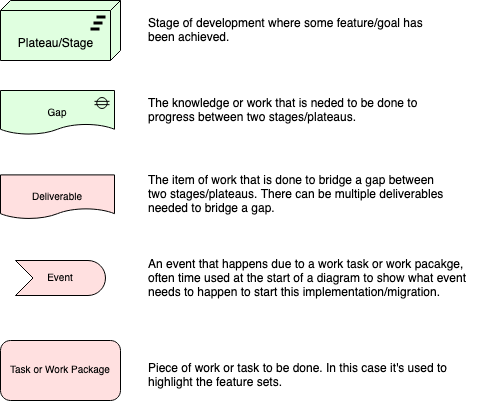
\includegraphics[width=6cm]{assets/migrationKey.drawio.png}
    \caption{Implementation and migration diagram components (The open group, 2016 and Jonkers et al, 2011).}
    \label{fig:migrationKey}
  \end{figure}

  \newpage

  \begin{landscape}
    \begin{figure}
      \centering
      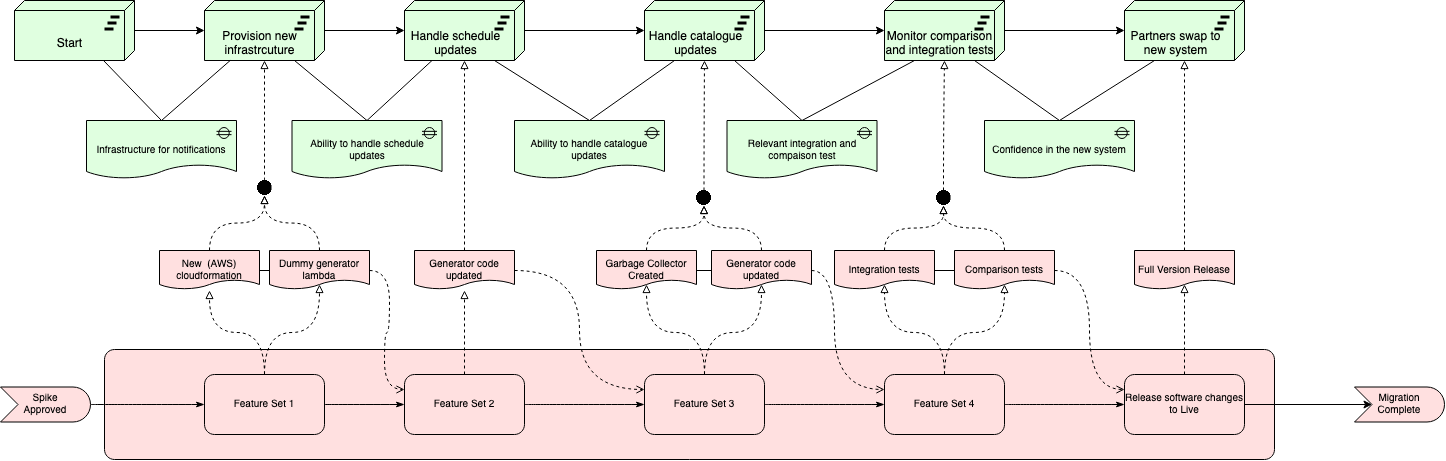
\includegraphics[width=20cm]{assets/migration.drawio.png}
      \caption{Figure showing Archimate implementation/migration diagram for project.}
      \label{fig:migration}
    \end{figure}
  \end{landscape}

  \newpage
  \subsection{Build software}
  Before discussing the build stage, it's important to understand the multiple environments used in development.

  \begin{figure}[H]
    \centering
    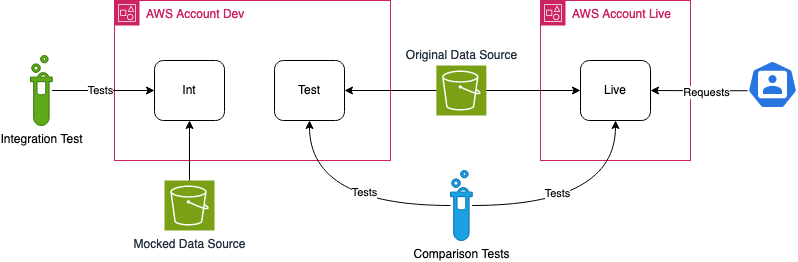
\includegraphics[width=8cm]{assets/environments.drawio.png}
    \caption{Diagram showing the different environments used by SpaceChimp.}
    \label{fig:environments}
  \end{figure}

  The above figure illustrates where the pipelines get their data from dependant on the environment, as well as what tests access said environment.
  We have 3 environments, int, test and live, with test mimicking live (Wiggins, 2017). This allows us to use the test environment to protect live from 
  any bugs or errors introduced by a task whilst also allowing the testing of outputs between old and software (Zheng, 2021). However when running on test
  and live we don't have control over the data source and the events it sends out to the pipeline, thus making it hard to test certain scenarios and features.
  This is where the int environment is used, we mock the data source used on test/live but have full control over what is added and removed, This allows 
  us to routinely check all edge cases and features are working as expected.

  \vspace{0.2cm}

  The build stage consists of writing and testing the software and resembles the flow of our kanban board.

  \begin{figure}[H]
    \centering
    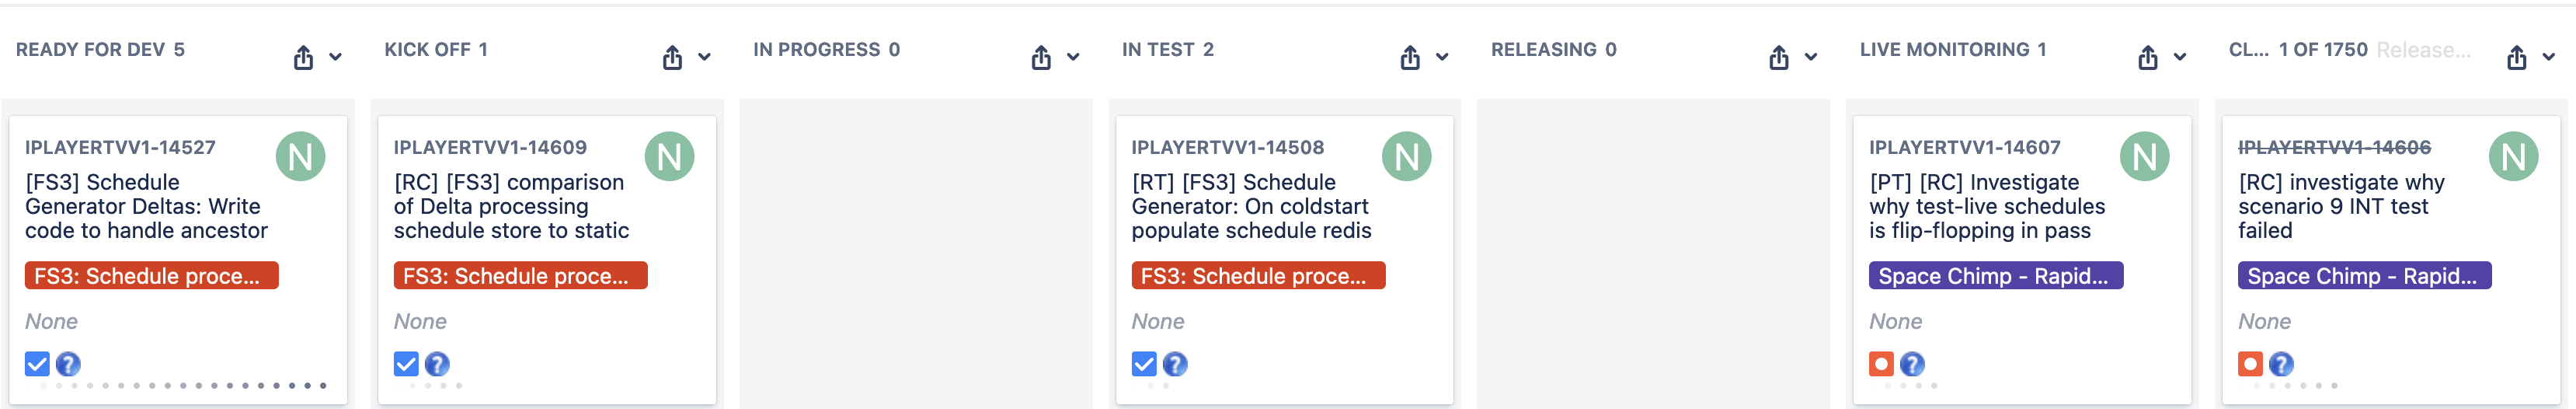
\includegraphics[width=10cm]{assets/kanbanBoard.png}
    \caption{SpaceChimps kanban board.}
    \label{fig:kanbanBoard2}
  \end{figure}

  \begin{itemize}
    \item \textbf{Ready for dev} - Tasks that are ready to be picked up for development.
    \item \textbf{Kick-off} - Tasks that need a test kick-off, which is not the same as the previous sections kick-off. This is where developers
    discuss the task with a member of the test team and determine the Acceptance Criteria (ACs) and test approach for the task.
    \item \textbf{In Progress} - Tasks that are being developed and worked on.
    \item \textbf{In Test} - Task has been completed and changes are on the test environment. A member of the test team can now test the ticket
    based on the previous discussions had in the kick-off. If things have changed during development, an additional hand-over with the test team 
    is done to discuss the new changes.
    \item \textbf{Releasing} - After a ticket task has been tested and has met the specified ACs, the task is moved to the releasing column signifying 
    that is ready to be deployed to the live environment.
    \item \textbf{Live monitoring} - Tasks in this column need to be monitored on the live environment to make sure that the change is functioning as expected.
  \end{itemize}

  \begin{figure}[H]
    \centering
    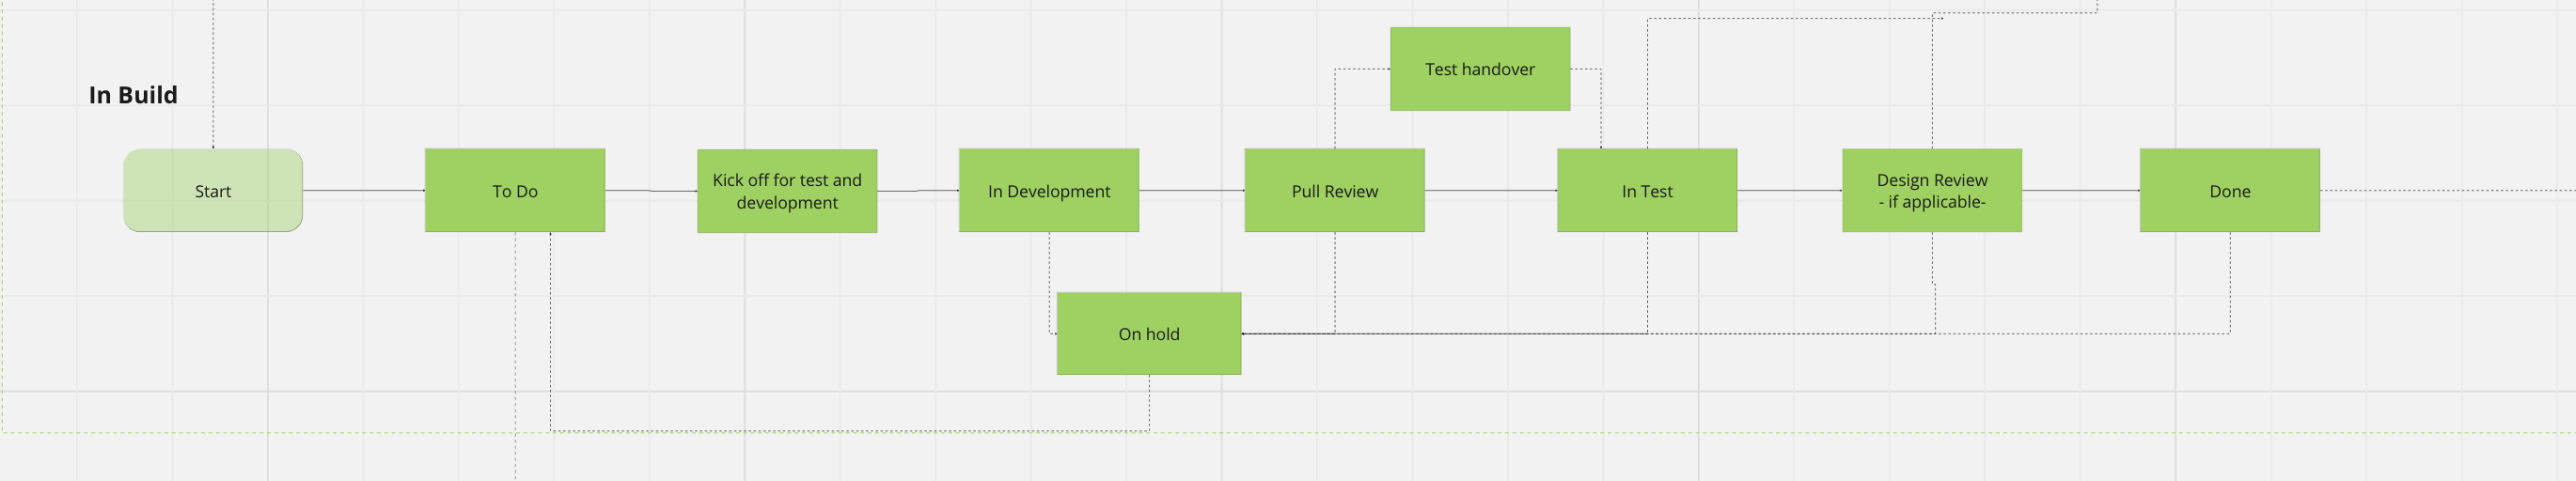
\includegraphics[width=8cm]{assets/workflow/build.png}
    \caption{Build stage of our of working.}
    \label{fig:workflowBuild}
  \end{figure}

  I will now discuss the 4 key components/features that were built during this stage, along with decisions and challenges that occurred during development.

  \newpage
  \subsubsection{Delta/change lambda}


  \newpage
  \subsubsection{Coldstarts}
  We use the term coldstart to refer to the refreshing of all data, in schedules terms all schedules will be checked to see if an update has occurred.
  This is not related to a cold start/boot in relation to serverless architectures (Microsoft Azure, 2018), although this is something that can affect 
  our lambdas. We already had a coldstart in place but changes would have to be made to work with the new delta/notifications environment.

  \begin{figure}[H]
    \centering
    \includegraphics[width=8cm]{diagrams/activity/Intial Coldstart Design.png}
    \caption{Activity diagram showing initial idea for coldstart changes.}
    \label{fig:initialColdstart}
  \end{figure}

  The above diagram shows the initial design for how the coldstart would function. The changes seem relatively simple:
  \begin{enumerate}
    \item Disable triggering of lambda on delta notification event. This is so no changes can interfere with the refresh of data.
    \item Purge the queue of updates before starting processing to stop unnecessary triggers of the lambda after the cold start has finished.
    \item Populate the redis with all the catalogue data it needs, this is done on schedule updates also. 
    \item Re-enable the triggering of lambda on delta notification event.
  \end{enumerate}

  Disabling and enabling of the lambda trigger can be achieved through the UpdateEventSourceMapping api (Amazon Web Services, 2024l) provided by AWS. 
  At the start, the trigger can be disabled, then re-enabled once the coldstart is finished.

  \begin{figure}[H]
    \centering
    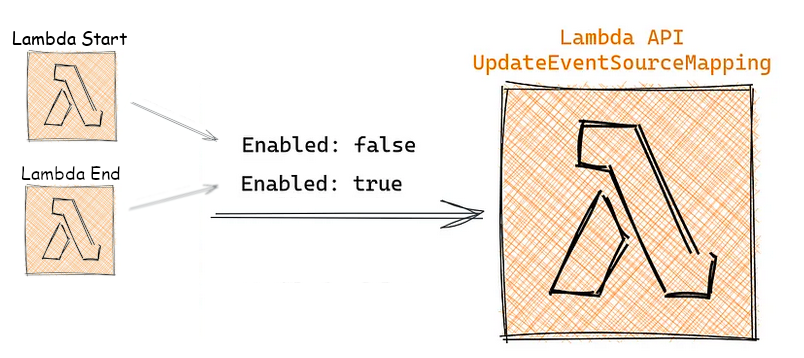
\includegraphics[width=8cm]{assets/lambdaMapping.png}
    \caption{Diagram edited from Charles (2021) to show lambda mapping states.}
    \label{fig:lambdaMapping}
  \end{figure}

  Purging the SQS queue of delta notifications can also be done though a similar API and the population of redis is already done per schedule, so 
  this seems like an easy switchover to work in the new world of delta notifications.

  However, as work began the code grew more and more complex, due mainly to the new logic of copying data over into the new schedule redis keyspace.
  Maintaining the broadcast list in the episodes would mean making the population logic complex and hard to follow. Code complexity can be a huge 
  problem with developers not wanting to edit the code in fear of breaking the current workings, difficulty to maintain 
  (Mateus, Andre, 2022 and Olbrich et al, 2009) and the \textit{truck/bus factor} which illustrates how hard it would be for a new team member to 
  understand with no help from the creator (Avelino et al, 2016). In addition to this, a study done by (Taibi et al, 2017) found that 
  \textit{'Smells related to size and complexity are considered harmful by a higher percentage of participants than others.'}. The system created is 
  complex and has multiple inputs that can interfere with each other, the same study also found that this higher complexity is less likely to be 
  refactored in the future (Taibi et al, 2017).

\begin{table}[H]
  \centering
  \begin{tabular}{|l|llr|}
  \hline
  \multicolumn{1}{|c|}{\multirow{2}{*}{Complexity}} & \multicolumn{3}{l|}{Level of occurrence (\%)}                        \\ \cline{2-4} 
  \multicolumn{1}{|c|}{}                            & \multicolumn{1}{l|}{Seldom} & \multicolumn{1}{l|}{Regularly} & Often \\ \hline
  Low                                               & \multicolumn{1}{l|}{7.94}   & \multicolumn{1}{l|}{23.81}     & 57.14 \\ \hline
  Medium                                            & \multicolumn{1}{l|}{12.70}  & \multicolumn{1}{l|}{55.56}     & 19.05 \\ \hline
  High                                              & \multicolumn{1}{l|}{46.03}  & \multicolumn{1}{l|}{28.57}     & 14.29 \\ \hline
  \end{tabular}
  \end{table}

  For these reasons a new approach was thought of. The coldstart would tidy up the differences between it's \textit{truth} the internal store, and 
  it's output. Anything not in the internal store is to be removed with the rest of the schedules being processed as if it was a delta notification 
  event.

  \begin{figure}[H]
    \centering
    \includegraphics[width=8cm]{diagrams/sequence/Final Coldstart.png}
    \caption{Sequence diagram showing the new flow of the final coldstart solution.}
    \label{fig:finalColdstart}
  \end{figure}

  This allows the re-use of existing code whilst reducing the complexity and potential code duplication of the coldstart by a sizeable amount.

  \newpage
  \subsubsection{Garbage Collector}
  Nowadays garbage collectors are synonymous with programming languages such as Java (Xu et al, 2019), however the first language to implement garbage 
  collection was LISP in the 1960s (Matam, 2023). Before then programmers had to manually assign memory for variables stored on the heap, as well as 
  unassign the memory when they were finished using it (Fakhoury et al, 2024 and Matam, 2023). 
  Garbage collection stops memory leaks as any unused memory is reclaimed (Microsoft, 2023).

  Whilst doing the spike it was thought that a form of \textit{garbage collector} may help simplify some of the logic around the removal of catalogue items
  from redis. Episode were easy to remove as once their associated broadcast list was empty they no longer needed to be stored. But due to having to 
  traverse upwards to find other linked items, it became complex and time consuming to calculate if an episodes parents (series) and grandparents (brands)
  also needed to be removed from the schedule redis store.

  \begin{figure}[H]
    \centering
    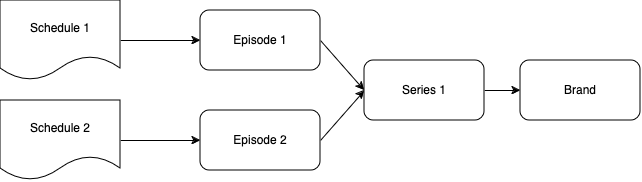
\includegraphics[width=8cm]{assets/catalogueTree.drawio.png}
    \caption{Example tree and associations between objects.}
    \label{fig:catalogueTree}
  \end{figure}

  Looking at the figure above outlines one possible scenario. If \emph{Episode 1} is removed from \emph{Schedule 1} then the episode object should be removed
  from redis and so should it's parent \emph{Series 1} as that also no longer has any schedule relations. However \emph{Brand} must stay as it still
  has \emph{Episode 2} and \emph{Series 2} that depend on it and relate it to \emph{Schedule 2}. Due to the potential to fan out like this, all data stored
  in the redis keyspace would have to be checked to see if there was any schedule still depending on the top level object (the brand). This takes a lot of
  memory and bandwidth to retrieve all this data. It was for that reason that it was decided, once a day a garbage collector should be ran to 
  tidy up anything no longer required.

  \begin{figure}[H]
    \centering
    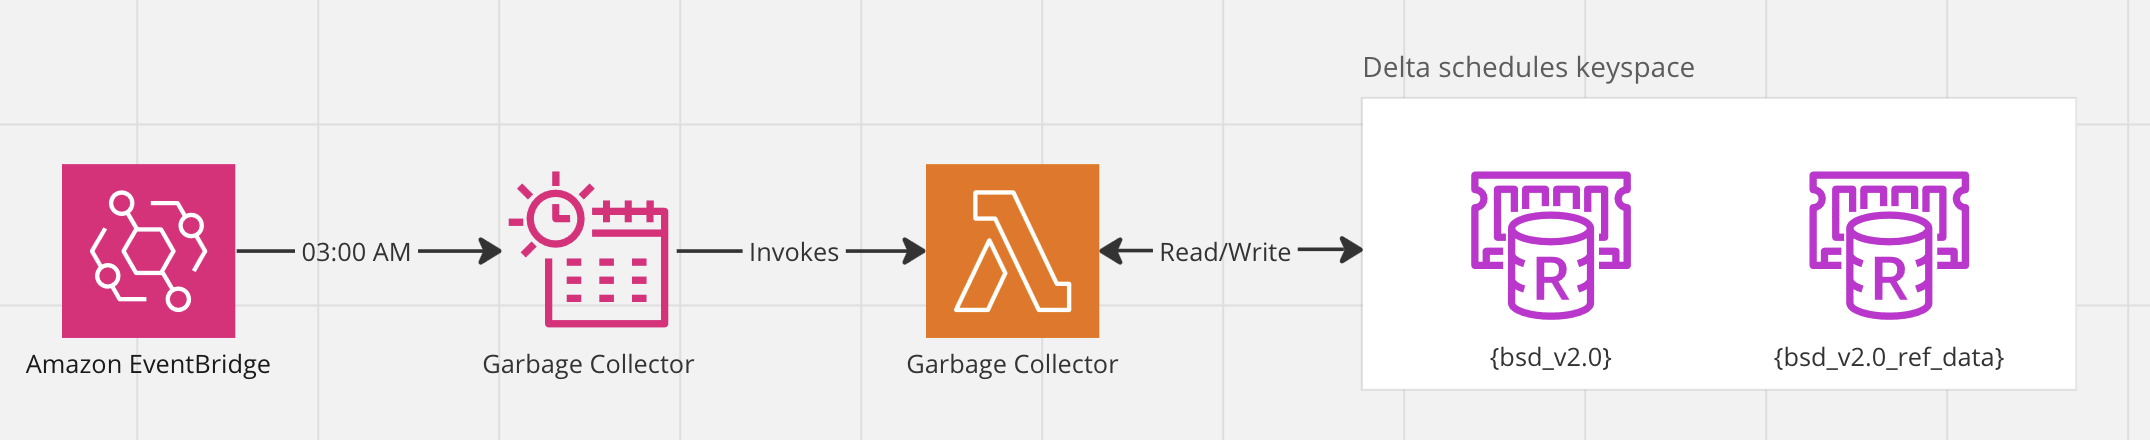
\includegraphics[width=8cm]{assets/architectures/garbageCollector.png}
    \caption{Garbage collector architecture.}
    \label{fig:garbageCollectorArchitecture}
  \end{figure}

  Above is the final architecture, a lambda is triggered by a scheduler once a day a 3AM to tidy up the leftover series and brands. In a later
  \hyperref[sec:garbageCollectorConsolidation]{\textbf{section}} the idea of moving all catalogue removals, including episodes, to the garbage 
  collector is explored.

  \newpage
  \subsubsection{End-to-end tests}
  In this section I want to discuss the larger tests that were created as part of the project. These include end-to-end (e2e) and comparison tests.
  As a team we follow the pattern of tests layed out in the test pyramid.

  \begin{figure}[H]
    \centering
    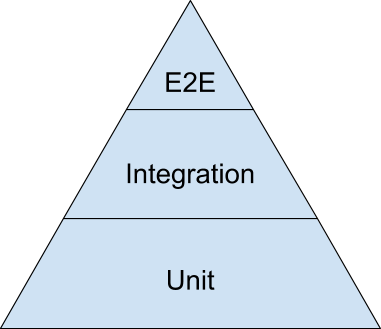
\includegraphics[width=6cm]{assets/testPyramid.png}
    \caption{Test pyramid (Wacker, 2015).}
    \label{fig:testPyramid}
  \end{figure}

  Unit tests and integration tests are written alongside the code, and can run on project build as they are cheap and quick to run (Spinellis, 2017).
  E2e tests sit at the top of this pyramid and should be used sparingly. This is not always the case, in other types of development, for example mobile,
  this pyramid can be turned upside down (Knott, 2015, cited in Contan, Dehelean and Miclea, 2018). This is probably due to mobile application being 
  primarily UI driven, which is the opposite for this project.

  In addition to this e2e and integration tests often get confused with one another. Integration tests \textit{'ensure synchronization between modules'}
  (Testim, 2021), and are more comparable to a unit test. Whereas a unit test is concerned on a single function/method an integration would test the calling of 
  methods by other methods and ensure integration between these two functions are working as expected. E2e tests are focused on actions/events that the 
  system must deal with as normal operation and could be described as automated manual testing (Testim, 2021).
  
  Due to their higher complexity, e2e tests are not without their potential problems. These include maintenance the written 
  tests, flakiness (are prone to randomly pass or fail without any discernable reason), time taken to run the tests and the cost of both the 
  execution of the tests and the time to write them (Yang and Leotta et al, 2023). 

  One of the larger problems we've faced in the passed is asynchronicity between tests (Leotta et al, 2023). For example if we upload a schedule at the 
  start of the pipeline and want to test it's structure at the end of the pipeline where partners would receive it, there's a lot that can interfere with 
  expected outputs. For the most part these bugs are when tidy up of a previous test is not carried out fully. If two test use the same identifier 
  for a schedule and then don't remove said schedule, this can result in tests not running how expected. It's for this reason during the development 
  of these new tests the code below was written to ensure that the schedule item about to be asserted on is not stored in the redis prior to the 
  test starting.

  \begin{lstlisting}[caption=Code to ensure schedule to asserted on is not present at the start of the test.]
    waitFor(`Ensure ${schedule} is not present before running test`, async () => {
      const bsd = await fetchFromRedis({
        command: 'isAbsent',
        keySpace: 'bsd_v2.0',
        sidDates: [schedule],
      })
      expect(bsd).toEqual([null])
    })
  \end{lstlisting} 

  Our current tests are written in \textit{scenarios} by our test team, a list of which can be seen in \hyperref[sec:AppendixF]{\textbf{Appendix F}}.
  Currently these cover all possible scenarios, however have a lot of overlap and repetitiveness. In an ideal world a test would cover an individual
  use case (Daly, 2022). These 14 scenarios could then be a part of these use case tests which would speed how quickly they run, thus lowering the cost.
  These use cases could be the following:

  \begin{itemize}
    \item Update a schedule
    \item Delete a schedule
    \item Update an episode
    \item Update an ancestor (series/brand)
    \item Tidy up orphaned items in redis (garbage collector)
  \end{itemize}

  This lowers the number of running test by 9 and removes a lot of time and duplication taken by setting up the scenarios. Due to time constraints and 
  prioritisation of other projects for the future, this refactor has not yet been undertaken but is in the backlog of things to do in the future. The 
  cost saved from changing this wouldn't be high, and doesn't justify the time it would take to refactor.

  For this project we stuck with the scenarios, some had already been done in previous work which meant we only had tests to write for the new 
  notification functionality. After discussion with the test team these tests include:

  \begin{enumerate}
    \item Hydration of episode stub to full episode object on episode update, as well as the episode parents and grandparents being transferred. This
    test would also make sure any schedules associated with the episodes titling was updated.
    \item Complex logic on schedule update, when a broadcasts episode changes in the schedule, if that episode has no remaining links to any other 
    schedules it should be removed from the schedule redis.
    \item Test whether correct supplementary data matches what is in the schedule. For partner requests we also send episode/series/brand data, 
    this data should be relevant to the broadcasts contained within the schedule.
  \end{enumerate}

  There were originally more test scenarios to be done as part of this project. However after discussing with both developers and testers it was decided 
  that these were either already being tested by unit tests or other parts of the testing library, or were unnecessary. This work was removed from 
  the board which can be seen in the burn-up charts in the \hyperref[sec:burnup]{\textbf{Outputs}} section.

  Finally we created comparison tests, to compare the old static output and new delta/notification output. These tests could be compared to extract, 
  transform, load (ETL) testing (Talend Inc, 2024). These tests will give us the confidence to switch our partners over to the new system. We decided
  upon a 1 week time frame where these comparisons tests must pass continuously before we are happy to make the switch. On failure the logs from the test
  will help us debug any current and future issues with the system.
   
  \newpage
  \subsection{Release}
  The release stage is the final stage in our workflow. This is when software gets released to the live environment and becomes available to partners. 
  \begin{figure}[H]
    \centering
    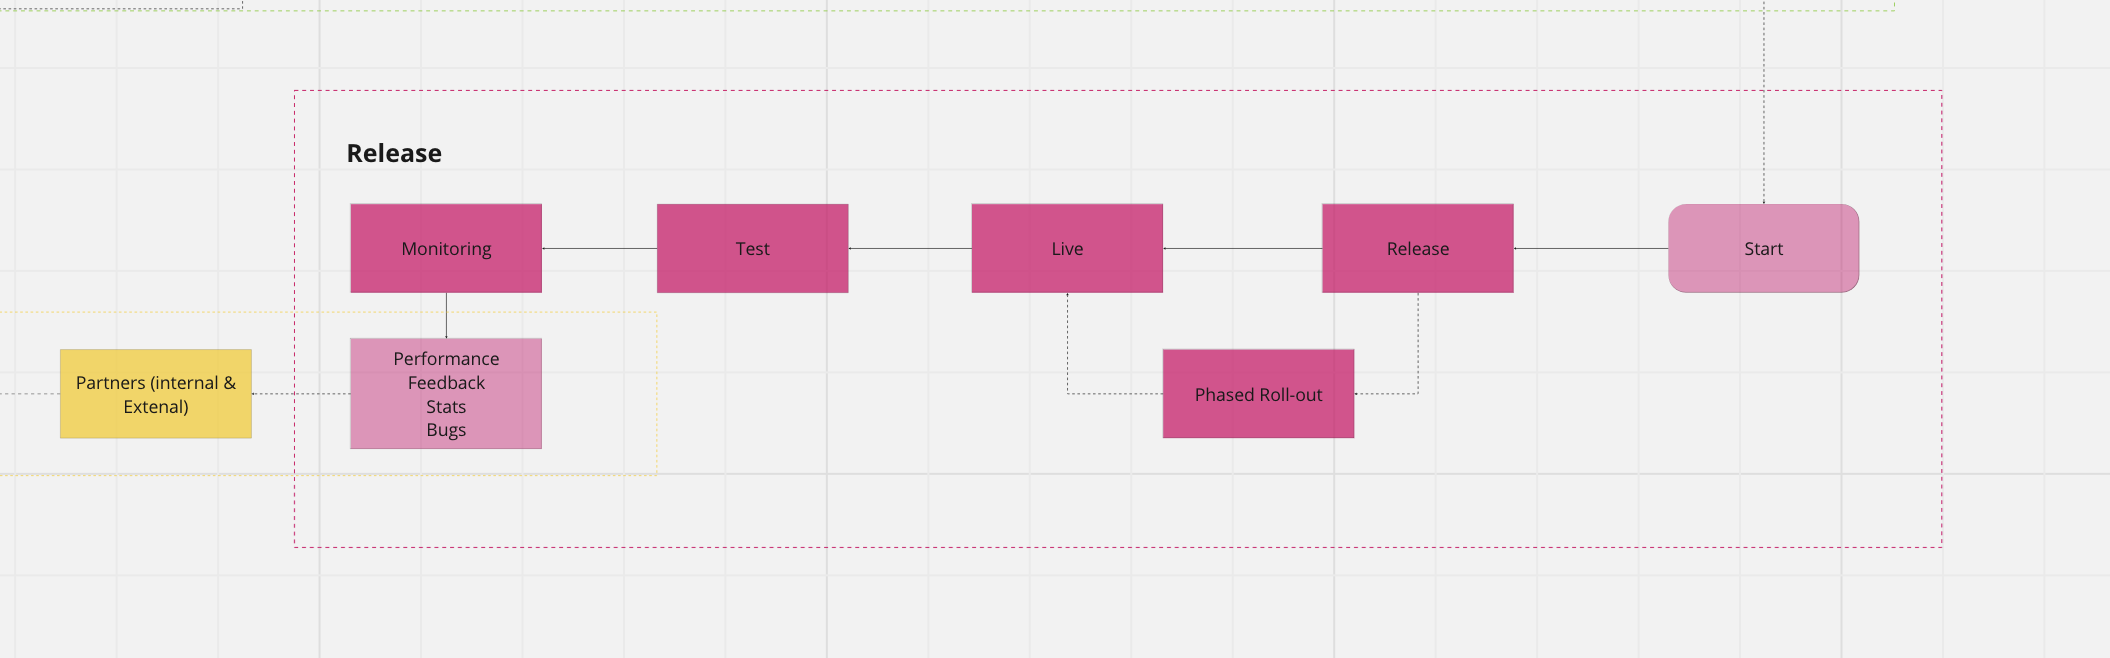
\includegraphics[width=8cm]{assets/workflow/release.png}
    \caption{Release stage of our ways of working.}
    \label{fig:workflowRelease}
  \end{figure}
  
  However in this case it doesn't become available to partners until we have confidence in the new system. We have config for each partner that 
  specifies what data they have access to. In the case of schedules, this includes keyspace information on where the data is retrieved from. As 
  previously discussed in the \hyperref[sec:cicd]{\textbf{Research}} section, the new and old system will run in parallel until our comparison tests 
  convince us that the new system outputs the same as the old.

  \begin{figure}[H]
    \centering
    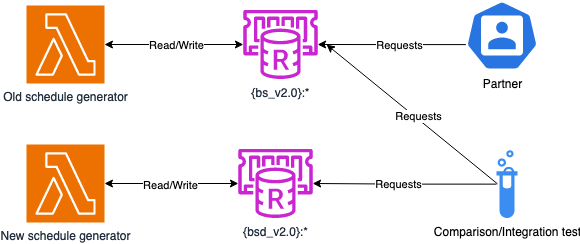
\includegraphics[width=8cm]{assets/keyspaceAccess.drawio.png}
    \caption{Diagram showing access to keyspaces.}
    \label{fig:keySpaceAccess}
  \end{figure}

  Until then partners will still access data from the old system, with a simple config change being the rollover/rollback mechanism. If we wanted we 
  could setup an automatic rollback and huddle system (Sathre, Zambreno, 2008), with the huddle portion consisting of developers being called out if 
  outside of working hours to monitor and remedy the situation. This can be done in many ways but one way would be through AWS alarm 
  actions (Amazon Web Services, 2024k). An alarm going into error would  triggers a rollback of the configs version in S3 (Amazon Web Services, 2024d).

  \begin{figure}[H]
    \centering
    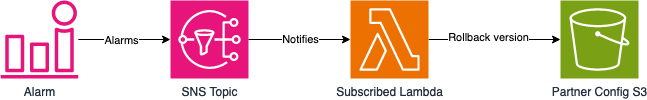
\includegraphics[width=8cm]{assets/rollback.drawio.png}
    \caption{Automatic rollback architecture on alarm error.}
    \label{fig:rollback}
  \end{figure}

  For our case this is most likely over-engineering and unnecessary. A config change only takes a minute to do and if there ever was an error we 
  would be notified and called out to fix the problem when necessary. 

  Once the switchover happens we wait for partner feedback and use created dashboards, these will be shown in the next section, to monitor 
  the new software. Alongside this, our comparison test and side-by-side running of new and old systems will continue for a short while after release, 
  allowing an easy rollback to the old system. Next this old lambdas scheduler will be disabled, but the lambda itself kept in case of an emergency. 
  Finally, after sufficient time has passed the old system can be deconstructed and removed completely.

\newpage

  \section{Outputs}

\newpage

  \section{Future Work and Conclusions}
\label{sec:future}
This report has discussed the creation and upgrade of an enterprise system that will be used by millions of people across the UK.

\begin{figure}[H]
  \centering
  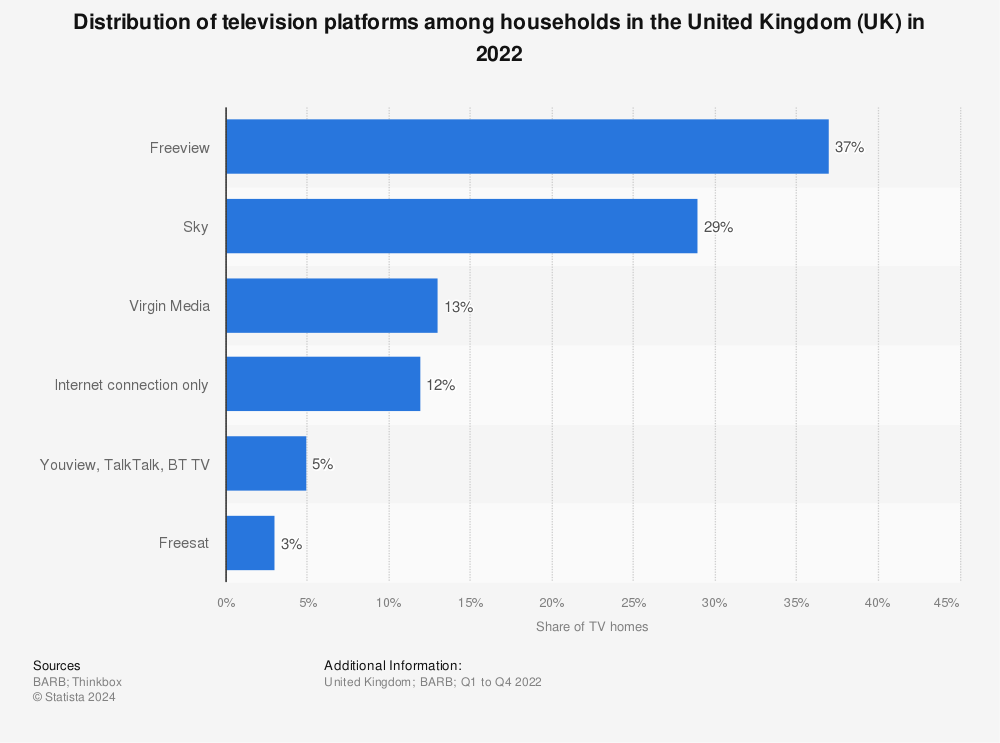
\includegraphics[width=8cm]{assets/tvPlatformChart.png}
  \caption{Chart showing freeview, a partner using the schedule feed, having the highest usage in UK homes (Statista, 2022).}
  \label{fig:tvPlatformChart}
\end{figure}

The report covered all parts of the software development life cycle (SDLC), including requirements, business drivers for the project, research,
a spike of the initial design, creation of tasks and work slices for a development and test team to work on, the creation of the software and
finally, the releasing of this new software to a live system depended on by partners.

To finish off this report I will discuss three future upgrades that could be made to the schedules system to improve both its timeliness of data updates
and a way that the system can be parallelised and simplified.

\subsection{Notifications direct to partners}
The new system relies on partners requesting data in order to update their UIs. This can mean that partners interfaces are still out of date, even 
though our internal store is as up to date as possible.

\begin{figure}[H]
  \centering
  \includegraphics[width=6cm]{diagrams/sequence/How Partners Remain Out of Date.png}
  \caption{Sequence diagram showing how partners become out of date in new system.}
  \label{fig:sequenceOutOfDate}
\end{figure}

In addition to this, re-requesting schedules that haven't been updated is a waste of time and costs the organisation money for data 
transfers (Amazon Web Services, 2024g). Below is an architecture that attempts to solve this problem by directly sending notifications to 
partners when an update occurs.

\begin{figure}[H]
  \centering
  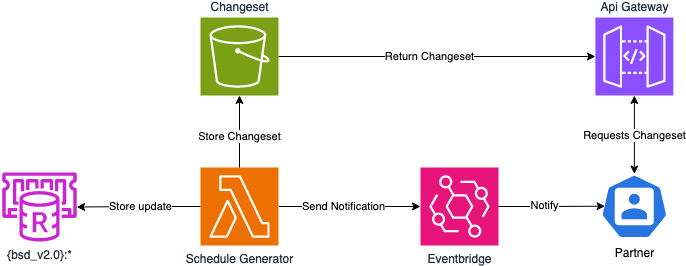
\includegraphics[width=10cm]{assets/architectures/changesets.drawio.png}
  \caption{Potential architecture to serve notifications to partners.}
  \label{fig:changsetArchitecture}
\end{figure}

A notification ID is sent to a partners system, they then request a \textit{'changeset'} from our API which consists of only the data that has been updated.
This new schedule can then be used instead of the old one, without doing a full refresh of all the schedules a client wants access to.

\begin{figure}[H]
  \centering
  \includegraphics[width=10cm]{diagrams/sequence/Changeset Lifecycle.png}
  \caption{How an schedules can be kept up to date using changesets.}
  \label{fig:changsetLifecycle}
\end{figure}

\newpage
\subsection{Parallelise the current system}
The new system is single-threaded and is unable to run in parallel due to shared memory between the threads needing to be managed. The piece of memory
at fault here is the broadcast list held in episodes that link that episode to schedules in which it is referenced. The main problem here is redis 
can't help us with any form of locking, unless we implement it ourselves, more on this can be found in the \hyperref[sec:storageSolutions]{\textbf{Research}}
section of this report.

During this research DynamoDB came up as a possible solution due to it's use of optimistic locking capabilities 
(Kanungo, Morena, 2023 and Amazon Web Services 2024h). Using a column to monitor for changes, code could be written using Amazons Software Development
Kit (SDK) (IBM Cloud Education, 2021) to ensure that no changes had occurred to the underlying before writing to the table. 

\begin{table}[H]
  \centering
  \begin{tabular}{|p{0.3\textwidth}|p{0.4\textwidth}|p{0.3\textwidth}|}
    \hline
    ID & Associations & Version \\ \hline
    Unique identifier of of the object which would be used for quick lookups. 
    & For series and brand objects this would be a list of children (series/episode) that the object refers to. Foe episodes this would now be 
    where the broadcast list of related schedules is stored.
    & Number that is used to determine if changes have occurred using optimistic locking. This will be incremented by 1 every time a change happens. \\ \hline
  \end{tabular}
  \caption{Example of dynamoDB table columns that could be used.}
\end{table}

This table can be combined with the following SDK command to optimistically lock the data being edited. In this code \emph{ConditionExpression} is 
the argument that determines what row is locking the record.

\begin{lstlisting}[caption=SDK command sent to optimistically lock writes to the assocaitions column.]
  const updateCommand = new UpdateItemCommand({
    TableName: 'schedule-associations',
    Key: marshall({ id: objectIdToUpdate }),
    UpdateExpression: 'set associations :newAssociations',
    ConditionExpression: 'version = :previousVersion',
    ExpressionAttributeValues: marshall({ 
      ':newAssociations': newAssociations,
      ':previousVersion': initialObject.version 
    })
  })
  \end{lstlisting}

  Finally this can all be integrated into a new architecture that is outlined below.

  \begin{figure}[H]
    \centering
    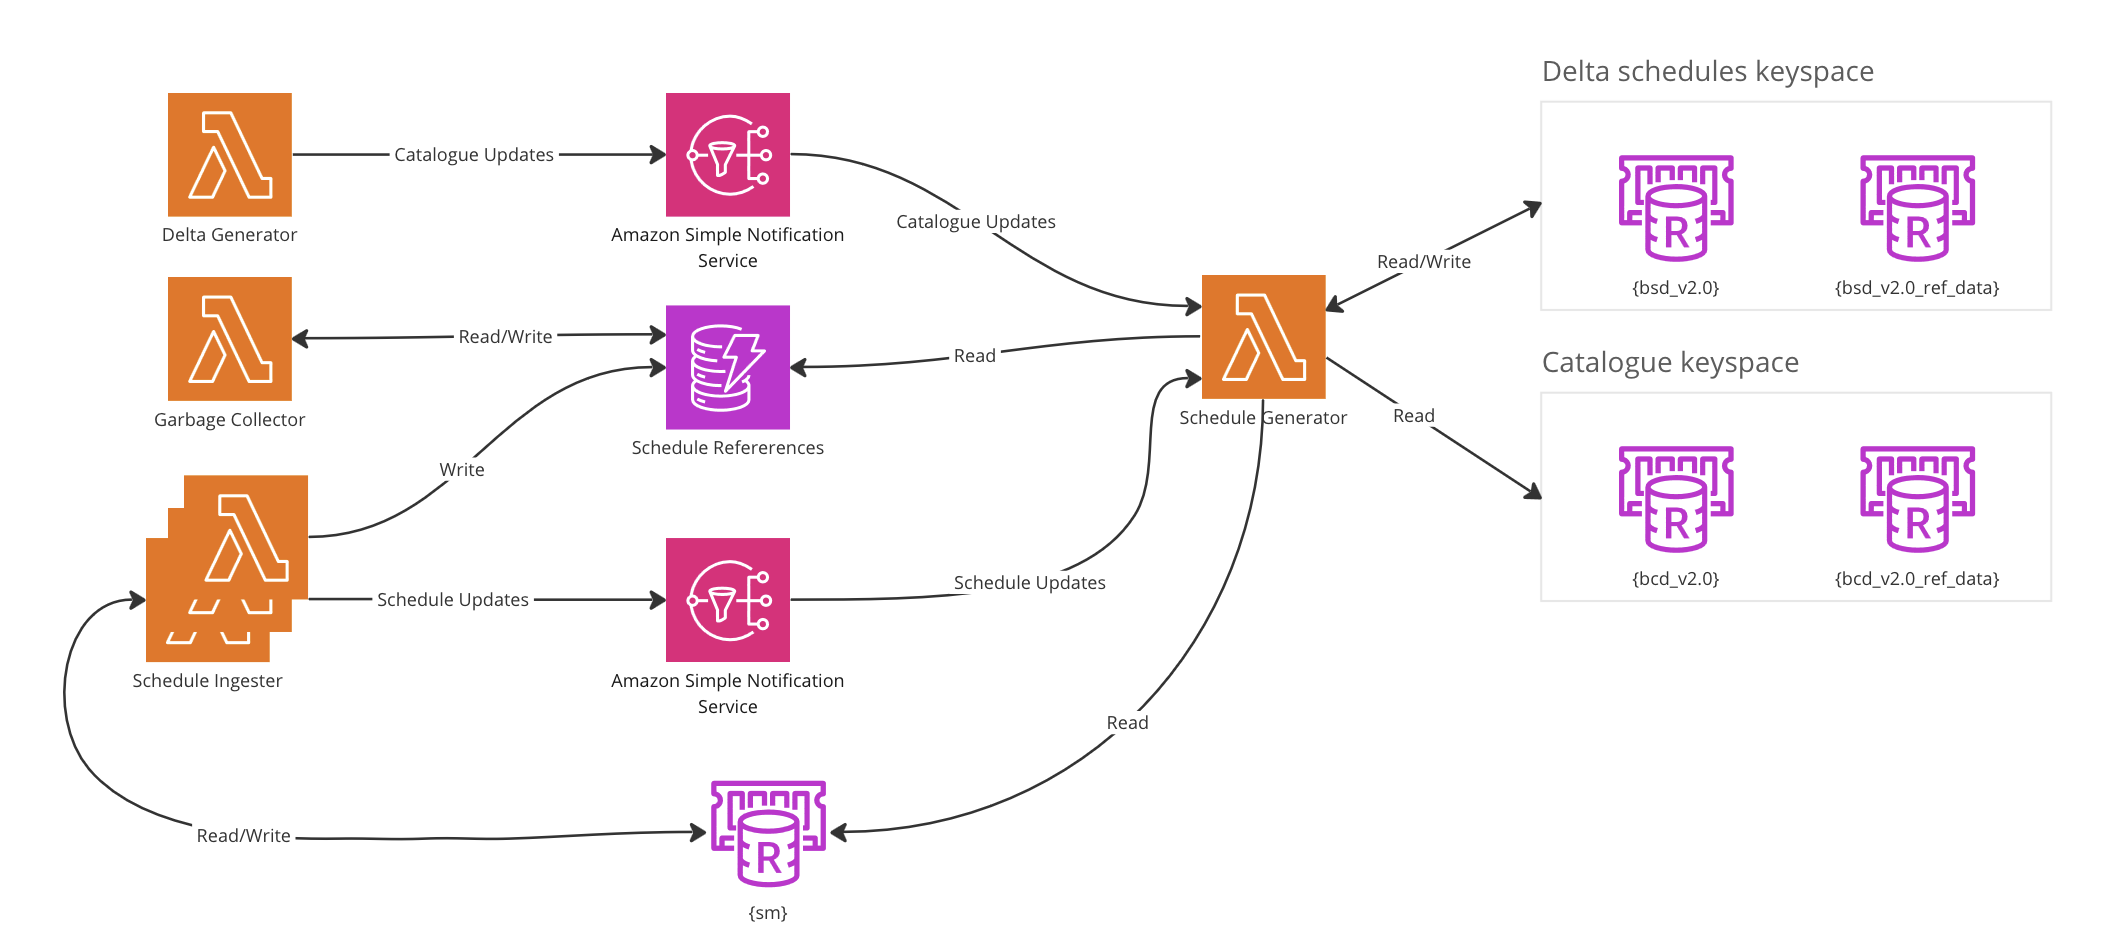
\includegraphics[width=10cm]{assets/architectures/dynamo.png}
    \caption{Option for parallelised architecture.}
    \label{fig:dynamoArchitecture}
  \end{figure}

  The system still takes input from both the schedule ingester and catalogue pipeline as before. However the aforementioned dynamoDB table is populated 
  by ingester and the catalogue pipeline, with the schedule generator no longer needing access to that data. Instead an AWS pipe (Amazon Web Services, 2024i) 
  is used to trigger invocation of the delta lambda for catalogue updates, whilst schedule updates function the same. AWS pipes consist of 4 sections:

  \begin{enumerate}
    \item \textbf{Source} - DynamoDB streams can be used as a source to a pipe (Amazon Web Services, 2024j), this stream representing a change to the table.
    This event can contain both old and new items from the dynamoDB table, as well as the type of event that it is (Silveria, 2020).
    \item \textbf{Filter} - We can filter out events based on the type of change made, we only want to trigger a lambda invocation on a MODIFY and not 
    on an INSERT or DELETE as these events are covered by the standard schedule processing.
    \item \textbf{Enrichment} - Not used in this example but can trigger extra enrichment of the data prior to the final target.
    \item \textbf{Target} - This is where to send the filtered data to. In this case it's the schedule generator itself.
  \end{enumerate}

  The inclusion of the dynamoDB table allows the use of optimistic locking to eventually parallelise the entire schedule pipeline. However there are 
  other huge benefits here as well with the highlights being:

  \begin{itemize}
    \item There is no longer a need to copy over catalogue data to the schedules redis store as it was only used to maintain the link between episode and 
    schedules via the broadcast list. This lowers the complexity of the schedule generator and allows the possibility for parallelism.
    \item The catalogue pipeline can be made to only send updates for objects that exist in schedules. 
      \begin{lstlisting}[caption=SDK command sent by catalogue pipeline to ignore non schedule related catalogue items.]
        const updateCommand = new UpdateItemCommand({
          TableName: 'schedule-associations',
          Key: marshall({ id: updatedCatalogueItem.id }),
          UpdateExpression: `set version ${initialObject.version + 1}`',
          ConditionExpression: `id = ${updatedCatalogueItem.id}`',
        })
      \end{lstlisting} 
      The above code once again uses the \emph{ConditionExpression}, but instead of optimistically locking here it is used to check if the objects exists.
      This works as if the object doesn't exists in the table it can't have an id. This will stop needless invocations of the schedule generator.
    \item An additional refinement stage could be added to the pipe to check that the modification to data that has happened would cause a change to a
    schedule. Only certain fields changes in catalogue items cause this so this could again save more invocations.
  
      \begin{figure}[H]
        \centering
        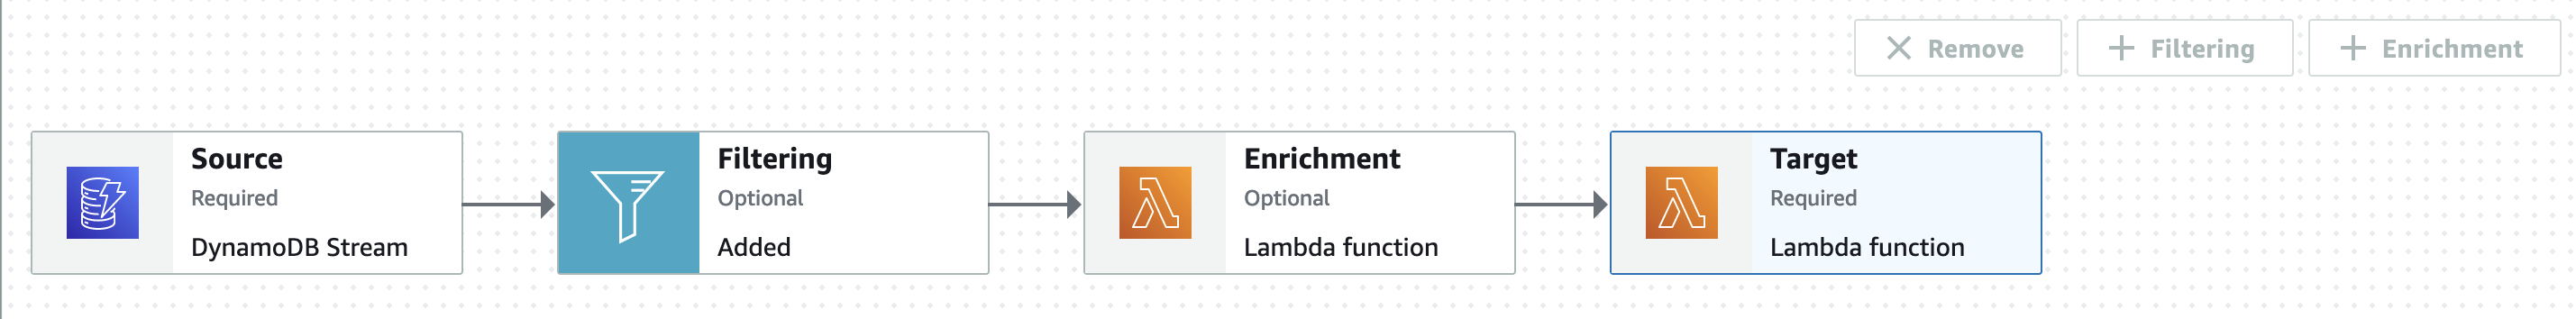
\includegraphics[width=12cm]{assets/awsPipeFull.png}
        \caption{AWS pipe including lambda enrichment stage.}
        \label{fig:awsPipeFull}
      \end{figure}
  \end{itemize}

  \newpage
  \subsection{Garbage Collection Consolidation}
  \label{sec:garbageCollectorConsolidation}

  A small change that could be made is for the garbage collector alone to handle removal of catalogue items, with the schedule generator only 
  removing schedules. This makes a lot of sense especially when applying the architectural principle of separation of concerns (SoC) which 
  \textit{'asserts that software should be separated based on the kinds of work it performs'} (Smith, 2023, ch. 3, p. 11). In addition to adhering 
  to well known principles it would also simplify what has become a bloated and complex schedule generator.

  The initial reason for removing the episode immediately upon deletion of schedule or the realisation that an episode was no longer referenced in 
  any schedule was for timeliness for partners. However this doesn't make sense, partners would never receive this orphaned information anyway due to 
  how the data is collected for them on request.

  \begin{figure}[H]
    \centering
    \includegraphics[width=6cm]{diagrams/activity/Partner Schedule Request.png}
    \caption{How supplementary catalogue data is calculated for partner request.}
    \label{fig:partnerRequest}
  \end{figure}  

  The benefits of removing this make things much clearer and is a quick win in comparison to some of the other suggestions for future work.

  \newpage
  \subsection{Conclusions}
  \label{sec:conclusion}
  
\newpage

  \section{References}

\noindent BBC. (2022) \textit{Timeline - History of the BBC} [online]. Available at \url{https://www.bbc.co.uk/historyofthebbc/bbc-100/timeline/} (accessed on 18th January 2024).
\vspace{0.2cm}

\noindent Pilnick, C. Baer, S, W. (1973) \textit{Cable television: A guide to the technology} [online]. Available at \url{https://www.rand.org/content/dam/rand/pubs/reports/2006/R1141.pdf} (accessed on 18th January 2024).
\vspace{0.2cm}

\noindent Ofcom. (2023) \textit{Media Nations report 2023} [online]. Available at \url{https://www.ofcom.org.uk/__data/assets/pdf_file/0029/265376/media-nations-report-2023.pdf} (accessed on 18th January 2024).
\vspace{0.2cm}

\noindent Ampere Analysis. (2023) \textit{Almost half of Internet users say they have switched off broadcast TV} [online]. Available at \url{https://www.ampereanalysis.com/press/release/dl/almost-half-of-internet-users-say-they-have-switched-off-broadcast-tv} (accessed on 18th January 2024).
\vspace{0.2cm}

\noindent Statista. (2023) \textit{Household penetration of smart TV sets in the United Kingdom (UK) from 2014 to 2023} [online]. Available at \url{https://www.statista.com/statistics/654074/smart-tv-penetration-in-uk-households/} (accessed on 18th January 2024).
\vspace{0.2cm}

\noindent Line Graph Maker. (2023) \textit{Bar Graph Maker} [online]. Available at \url{https://linegraphmaker.co/bar-graph} (accessed on 19th January 2024).
\vspace{0.2cm}

\noindent Amazon. (2021) \textit{Linear TV Integration Guide Overview} [online]. Available at \url{https://developer.amazon.com/docs/fire-tv/linear-tv-integration-guide-overview.html} (accessed on 18th January 2024).
\vspace{0.2cm}

\noindent Davie, T. (2022) \textit{A digital-first BBC} [online]. Available at \url{https://www.bbc.co.uk/mediacentre/speeches/2022/digital-first-bbc-director-general-tim-davie} (accessed on 18th January 2024).
\vspace{0.2cm}

\noindent Sparks, R. (2024) \textit{OKRs: the ultimate guide to objectives and key results} [online]. Available at \url{https://www.atlassian.com/agile/agile-at-scale/okr} (accessed on 18th January 2024).
\vspace{0.2cm}

\noindent Bowker O. (2023) \textit{Analysis of BBC process and proposal for a new API key management system}. Assignment for DC4000, MSc Digital and Technology Solutions Specialist, Aston University, Unpublished.
\vspace{0.2cm}

\noindent BBC Partnerships. (2023) \textit{Partnerships - one year on}. BBC. Unpublished.
\vspace{0.2cm}

\noindent Somerville, I. (2016) \textit{Software engineering}. Tenth edition, Global edition. London: Pearson Education.
\vspace{0.2cm}

\noindent Somerville, I. (2021) \textit{Engineering Software Products: An Introduction to Modern Software Engineering}. Global edition. London: Pearson Education.
\vspace{0.2cm}

\noindent Amazon Web Services. (2024a) \textit{AWS Lambda} [online]. Available at \url{https://aws.amazon.com/lambda/} (accessed on 2nd February 2024).
\vspace{0.2cm}

\noindent Amazon Web Services. (2024b) \textit{Amazon Simple Notification Service} [online]. Available at \url{https://aws.amazon.com/sns/} (accessed on 2nd February 2024).
\vspace{0.2cm}

\noindent Amazon Web Services. (2024c) \textit{Amazon Simple Queue Service} [online]. Available at \url{https://aws.amazon.com/sqs/} (accessed on 2nd February 2024).
\vspace{0.2cm}

\noindent Amazon Web Services. (2024d) \textit{Amazon S3} [online]. Available at \url{https://aws.amazon.com/s3/} (accessed on 2nd February 2024).
\vspace{0.2cm}

\noindent Amazon Web Services. (2024e) \textit{Amazon DynamoDB} [online]. Available at \url{https://aws.amazon.com/dynamodb/} (accessed on 2nd February 2024).
\vspace{0.2cm}

\noindent Amazon Web Services. (2024f) \textit{Amazon ElastiCache} [online]. Available at \url{https://aws.amazon.com/elasticache/} (accessed on 9th February 2024).
\vspace{0.2cm}

\noindent Amazon Web Services. (2024g) \textit{How AWS Pricing Works} [online]. Available at \url{https://docs.aws.amazon.com/pdfs/whitepapers/latest/how-aws-pricing-works/how-aws-pricing-works.pdf} (accessed on 20th February 2024).
\vspace{0.2cm}

\noindent Amazon Web Services. (2024h) \textit{Optimistic locking with version number} [online]. Available at \url{https://docs.aws.amazon.com/amazondynamodb/latest/developerguide/DynamoDBMapper.OptimisticLocking.html} (accessed on 21st February 2024).
\vspace{0.2cm}

\noindent Amazon Web Services. (2024i) \textit{Amazon EventBridge Pipes} [online]. Available at \url{https://aws.amazon.com/eventbridge/pipes/} (accessed on 20th February 2024).
\vspace{0.2cm}

\noindent Amazon Web Services. (2024j) \textit{Amazon DynamoDB stream as a source} [online]. Available at \url{https://docs.aws.amazon.com/eventbridge/latest/userguide/eb-pipes-dynamodb.html} (accessed on 21st February 2024).
\vspace{0.2cm}

\noindent Amazon Web Services. (2024k) \textit{PutMetricAlarm} [online]. Available at \url{https://docs.aws.amazon.com/AmazonCloudWatch/latest/APIReference/API_PutMetricAlarm.html#API_PutMetricAlarm_Errors} (accessed on 19th February 2024).
\vspace{0.2cm}

\noindent Amazon Web Services. (2024l) \textit{UpdateEventSourceMapping} [online]. Available at \url{https://docs.aws.amazon.com/lambda/latest/api/API_UpdateEventSourceMapping.html} (accessed on 23rd February 2024).
\vspace{0.2cm}

\noindent IBM. (2024) \textit{What is Redis?} [online]. Available at \url{https://www.ibm.com/topics/redis} (accessed on 9th February 2024).
\vspace{0.2cm}

\noindent IBM Cloud Education. (2021) \textit{SDK vs. API: What's the Difference?} [online]. Available at \url{https://www.ibm.com/blog/sdk-vs-api/} (accessed on 21st February 2024).
\vspace{0.2cm}

\noindent Redis Ltd. (2024a) \textit{Redis FAQ} [online]. Available at \url{https://redis.io/docs/get-started/faq/} (accessed on 9th February 2024).
\vspace{0.2cm}

\noindent Redis Ltd. (2024b) \textit{Redis pipelining} [online]. Available at \url{https://redis.io/docs/manual/pipelining/} (accessed on 9th February 2024).
\vspace{0.2cm}

\noindent Redis Ltd. (2024c) \textit{Transactions} [online]. Available at \url{https://redis.io/docs/interact/transactions/} (accessed on 9th February 2024).
\vspace{0.2cm}

\noindent Redis Ltd. (2024d) \textit{Redis modules and blocking commands} [online]. Available at \url{https://redis.io/docs/reference/modules/modules-blocking-ops/} (accessed on 9th February 2024).
\vspace{0.2cm}

\noindent Oracle Corporation. (2010) \textit{Defining Multithreading Terms} [online]. Available at \url{https://docs.oracle.com/cd/E19455-01/806-5257/6je9h032b/index.html} (accessed on 9th February 2024).
\vspace{0.2cm}

\noindent Eyng, R. (2019) \textit{Redis: Pipelining, Transactions and Lua Scripts} [online]. Available at \url{https://rafaeleyng.github.io/redis-pipelining-transactions-and-lua-scripts} (accessed on 9th February 2024).
\vspace{0.2cm}

\noindent Visual Paradigm. (2024) \textit{What is Spike in Scrum?} [online]. Available at \url{https://www.visual-paradigm.com/scrum/what-is-scrum-spike/} (accessed on 9th February 2024).
\vspace{0.2cm}

\noindent Ugarte, A. (2024) \textit{What Is Thread-Safety and How to Achieve It?} [online]. Available at \url{https://www.baeldung.com/java-thread-safety} (accessed on 9th February 2024).
\vspace{0.2cm}

\noindent Graefe, G. (2016) \textit{Revisiting optimistic and pessimistic concurrency control} [online]. Available at \url{https://www.labs.hpe.com/techreports/2016/HPE-2016-47.pdf} (accessed on 9th February 2024).
\vspace{0.2cm}

\noindent Thornton, G. (2001) \textit{Optimistic Locking with Concurrency in Oracle} [online]. Available at \url{https://www.orafaq.com/papers/locking.pdf} (accessed on 9th February 2024).
\vspace{0.2cm}

\noindent Weston, T. (2011) \textit{Optimistic and Pessimistic Concurrency Control with Shared Memory Models} [online]. Available at \url{https://baddotrobot.com/resources/concurrency-control-1.0-draft.pdf} (accessed on 9th February 2024).
\vspace{0.2cm}

\noindent Apache Software Corporation. (2013) \textit{Deadlocks} [online]. Available at \url{https://db.apache.org/derby/docs/10.0/manuals/develop/develop75.html} (accessed on 9th February 2024).
\vspace{0.2cm}

\noindent Heil, C. (2022) \textit{Is Kanban the better Agile Approach in a Highly-Regulated Environment?} [online]. Available at \url{https://www2.deloitte.com/content/dam/Deloitte/de/Documents/risk/Deloitte_Agile_Approach_in_Highly_Regulated_Environments.pdf} (accessed on 12th February 2024).
\vspace{0.2cm}

\noindent Rehkopf, M. (2024) \textit{Kanban vs. scrum: which agile are you?} [online]. Available at \url{https://www.atlassian.com/agile/kanban/kanban-vs-scrum} (accessed on 12th February 2024).
\vspace{0.2cm}

\noindent Mauvius Group Inc. (2021) \textit{The official guide to the kanban method} [online]. Available at \url{https://resources.kanban.university/wp-content/uploads/2021/06/The-Official-Kanban-Guide_A4.pdf} (accessed on 12th February 2024).
\vspace{0.2cm}

\noindent Jenkins. (2024) \textit{Pipeline Syntax} [online]. Available at \url{https://www.jenkins.io/doc/book/pipeline/syntax/} (accessed on 12th February 2024).
\vspace{0.2cm}

\noindent Rodriguez, P. Haghighatkhah, A. Lwakatare, L, E. Teppola, S. Suomalainen, T. Eskeli, J. Karvonen, T. Kuvaja, P. Verner, J, M. Oivo, M. (2017) 'Continuous Deployment of Software Intensive Products and Services: A Systematic Mapping Study', Journal of Systems and Software, Vol. 123, pp. 263-291. Available at: \url{https://doi.org/10.1016/j.jss.2015.12.015}
\vspace{0.2cm}

\noindent Taibi, D. Janes, A. Lenarduzzi, V. (2017) 'How developers perceive smells in source code: A replicated study', Information and Software Technology, Vol. 92, pp. 223-235. Available at: \url{https://doi.org/10.1016/j.infsof.2017.08.008}
\vspace{0.2cm}

\noindent Xu, L. Guo, T. Dou, W. Wang, W. Wei, J. (2019) 'An experimental evaluation of garbage collectors on big data applications', Proceedings of the VLDB Endowment, Volume 12, Issue 5, pp 570-583. Available at: \url{https://doi.org/10.14778/3303753.3303762}
\vspace{0.2cm}

\noindent Olbrich, S. Cruzes, S, D. Basili, V. Zazworka, N. (2009) 'The evolution and impact of code smells: A case study of two open source systems', 2009 3rd International Symposium on Empirical Software Engineering and Measurement. Available at: \url{https://doi.org/10.1109/ESEM.2009.5314231}
\vspace{0.2cm}

\noindent Mateus, L. Andre, H. (2022) 'How and why we end up with complex methods: a multi-language study', Empirical Software Engineering, Vol. 27, Issue 5, Article Number 115. Available at: \url{https://doi.org/10.1007/s10664-022-10144-3}
\vspace{0.2cm}

\noindent Avelino, G. Passos, L. Hora, A. Valente, T, M. (2016) 'A novel approach for estimating Truck Factors', 2016 IEEE 24th International Conference on Program Comprehension (ICPC). Available at: \url{https://doi.org/10.1109/ICPC.2016.7503718}
\vspace{0.2cm}

\noindent Department of Defence. (2021) \textit{DoD Enterprise DevSecOps Fundamentals} [online]. Available at \url{https://dodcio.defense.gov/Portals/0/Documents/Library/DoDEnterpriseDevSecOpsFundamentals.pdf} (accessed on 14th February 2024).
\vspace{0.2cm}

\noindent NSA. (2023) \textit{Defending Continuous Integration/Continuous Delivery (CI/CD) Environments} [online]. Available at \url{https://media.defense.gov/2023/Jun/28/2003249466/-1/-1/0/CSI_DEFENDING_CI_CD_ENVIRONMENTS.PDF} (accessed on 14th February 2024).
\vspace{0.2cm}

\noindent OWASP Foundation. (2023) \textit{OWASP Top 10 CI/CD Security Risks} [online]. Available at \url{https://owasp.org/www-project-top-10-ci-cd-security-risks/} (accessed on 14th February 2024).
\vspace{0.2cm}

\noindent Wikström, A. (2019) \textit{Benefits and challenges of Continuous Integration and Delivery - A Case Study} [online]. Available at \url{https://core.ac.uk/download/pdf/226768285.pdf} (accessed on 14th February 2024).
\vspace{0.2cm}

\noindent Fairbanks, J. Tharigonda, A. Eisty, N, U. (2023) \textit{Analyzing the Effects of CI/CD on Open Source Repositories in GitHub and GitLab} [online]. Available at \url{https://arxiv.org/pdf/2303.16393.pdf} (accessed on 14th February 2024).
\vspace{0.2cm}

\noindent GoRetro. (2023) \textit{Ways of Working} [online]. Available at \url{https://www.goretro.ai/glossary/ways-of-working} (accessed on 14th February 2024).
\vspace{0.2cm}

\noindent Banerjee, A. (2017) 'System Changeover Policy and Precautions', International Journal of Advanced Engineering and Management, Vol. 2, No. 9, pp. 214-218. Available at: \url{https://doi.org/10.24999/IJOAEM/02090048}
\vspace{0.2cm}

\noindent Smyth, D. (2020) \textit{Changeover Techniques} [online]. Available at \url{https://smallbusiness.chron.com/changeover-techniques-34890.html} (accessed on 15th February 2024).
\vspace{0.2cm}

\noindent IoRedis. (2024) \textit{README - ioredis} [online]. Available at \url{https://ioredis.readthedocs.io/en/stable/README/#transparent-key-prefixing} (accessed on 15th February 2024).
\vspace{0.2cm}

\noindent Rustagi, V. (2023) \textit{Strategies To Run Old \& new Systems Simultaneously Using The Same Database} [online]. Available at \url{https://metaorangedigital.com/blog/strategies-to-run-old-new-systems-simultaneously-using-the-same-database/} (accessed on 15th February 2024).
\vspace{0.2cm}

\noindent Bigelow, J, S. (2020) \textit{What are the types of requirements in software engineering?} [online]. Available at \url{https://www.techtarget.com/searchsoftwarequality/answer/What-are-requirements-types} (accessed on 16th February 2024).
\vspace{0.2cm}

\noindent Karolis, N, Saulius, G. (2023) 'Causal Knowledge Modelling for Agile Development of Enterprise Application Systems', Informatica (Netherlands), Vol. 34 Issue 1, p 124. Available at: \url{https://doi.org/10.15388/23-INFOR510}
\vspace{0.2cm}

\noindent Eduardo, M. (2022) 'Moscow Rules: A Quantitative Exposé', Lecture Notes in Business Information Processing, Vol. 445, pp 19-34. Available at: \url{https://doi.org/10.1007/978-3-031-08169-9_2}
\vspace{0.2cm}

\noindent Kim, M. Park, S. Sugumaran, V. Yang, H. (2007) 'Managing requirements conflicts in software product lines: A goal and scenario based approach', Data \& Knowledge Engineering, Vol. 61 Issue 3, pp 417-432. Available at: \url{https://doi.org/10.1016/j.datak.2006.06.009}
\vspace{0.2cm}

\noindent Kanungo, S, Morena, D, R. (2023) 'Concurrency versus consistency in NoSQL databases', Journal of Autonomous Intelligence, Vol. 7 Issue 3. Available at: \url{https://doi.org/10.32629/jai.v7i3.936}
\vspace{0.2cm}

\noindent Sanders, R. (1987), 'THE PARETO PRINCIPLE: ITS USE AND ABUSE', Journal of Services Marketing, Vol. 1 No. 2, pp. 37-40. Available at: \url{https://doi.org/10.1108/eb024706}
\vspace{0.2cm}

\noindent Hashimi, A, L. Gravell, A. (2020), 'Spikes in Agile Software Development: An Empirical Study', 2020 International Conference on Computational Science and Computational Intelligence (CSCI). Available at: \url{https://doi.org/10.1109/CSCI51800.2020.00319}
\vspace{0.2cm}

\noindent Hashimi, A, L. Abduldaem, A. Gravell, A. (2022), 'Common Spikes Success Factors: An Industrial Investigation within Agile Software Development', 2022 12th International Conference on Software Technology and Engineering (ICSTE). Available at: \url{https://doi.org/10.1109/ICSTE57415.2022.00008}
\vspace{0.2cm}

\noindent Hashimi, A, L. Gravell, A. (2019) 'A Critical Review of the Use of Spikes in Agile Software Development', The Fourteenth International Conference on Software Engineering Advances. Available at: \url{https://www.researchgate.net/publication/340446921_A_Critical_Review_of_the_Use_of_Spikes_in_Agile_Software_Development}
\vspace{0.2cm}

\noindent Spinellis, D. (2019) 'State-of-the-Art Software Testing', IEEE Software, Vol. 34, Issue 5, pp 4-6. Available at: \url{https://doi.org/10.1109/MS.2017.3571564}
\vspace{0.2cm}

\noindent Kruchten, P. Nord, L, R. Ozkaya, I. Visser, J. (2012) 'Technical Debt in Software Development: from Metaphor to Theory Report on the Third International Workshop on Managing Technical Debt', ACM SIGSOFT Software Engineering Notes Advances, Vol. 37, No. 5, p. 36. Available at: \url{https://doi.org/10.1145/2347696.2347698}
\vspace{0.2cm}

\noindent Sathre, J, Zambreno, J. (2008) 'Automated software attack recovery using rollback and huddle', Des Autom Embed Syst, Vol. 12, pp. 243-260. Available at: \url{https://doi.org/10.1007/s10617-008-9020-4}
\vspace{0.2cm}

\noindent Leotta, M. García, B. Ricca, F. Whitehead, J. (2023) 'Challenges of End-to-End Testing with Selenium WebDriver and How to Face Them: A Survey', 2023 IEEE Conference on Software Testing, Verification and Validation (ICST). Available at: \url{https://doi.org/10.1109/ICST57152.2023.00039}
\vspace{0.2cm}

\noindent Zheng, J. (2021) 'Research on software development and test environment automation based on association rules', 2021 IEEE International Conference on Emergency Science and Information Technology (ICESIT). Available at: \url{https://doi.org/10.1109/ICESIT53460.2021.9696910}
\vspace{0.2cm}

\noindent Burghate, N. (2018) 'Work Breakdown Structure: Simplifying Project Management', International Journal of Commerce and Management Studies (IJCAMS), Vol. 3, No. 2. Available at: \url{https://www.ijcams.com/wp-content/uploads/2018/06/WBS.pdf}
\vspace{0.2cm}

\noindent Contan, A. Dehelean, C. Miclea, L. (2018) 'Test automation pyramid from theory to practice', 2018 IEEE International Conference on Automation, Quality and Testing, Robotics (AQTR). Available at: \url{https://doi.org/10.1109/AQTR.2018.8402699}
\vspace{0.2cm}

\noindent Glas, T. Hedén, F. (2021) \textit{Managing Technical Debt in XP Teams} [online]. Available at \url{https://fileadmin.cs.lth.se/cs/Education/EDAN80/Reports/2021/GlasHeden.pdf} (accessed on 19th February 2024).
\vspace{0.2cm}

\noindent Microsoft. (2021) \textit{Technical Spike} [online]. Available at \url{https://microsoft.github.io/code-with-engineering-playbook/design/design-reviews/recipes/technical-spike/} (accessed on 19th February 2024).
\vspace{0.2cm}

\noindent Microsoft. (2023) \textit{Fundamentals of garbage collection} [online]. Available at \url{https://learn.microsoft.com/en-us/dotnet/standard/garbage-collection/fundamentals} (accessed on 23rd February 2024).
\vspace{0.2cm}

\noindent Martins, J. (2023) \textit{7 common causes of scope creep, and how to avoid them} [online]. Available at \url{https://asana.com/resources/what-is-scope-creep} (accessed on 19th February 2024).
\vspace{0.2cm}

\noindent Raeburn, A. (2024) \textit{The work breakdown structure (WBS) for project management: What it is and how to use it} [online]. Available at \url{https://asana.com/resources/work-breakdown-structure} (accessed on 19th February 2024).
\vspace{0.2cm}

\noindent The Open Group. (2016) \textit{Implementation and Migration Elements} [online]. Available at \url{https://pubs.opengroup.org/architecture/archimate30-doc/chap13.html#_Toc451758082} (accessed on 19th February 2024).
\vspace{0.2cm}

\noindent Jonkers, H. Proper, E. Lankhorst, M, M. Quartel, A, C, D. Iacob, M. (2011) 'ArchiMate(R) for Integrated Modelling Throughout the Architecture Development and Implementation Cycle', 2011 IEEE 13th Conference on Commerce and Enterprise Computing. Available at: \url{https://doi.org/10.1109/CEC.2011.52}
\vspace{0.2cm}

\noindent Fakhoury, R. Braginsky, A. Keidar, I. Zuriel, Y. (2024) 'Nova: Safe Off-Heap Memory Allocation and Reclamation', Leibniz International Proceedings in Informatics, Volume 286, Article number 15. Available at: \url{https://doi.org/10.4230/LIPIcs.OPODIS.2023.15}
\vspace{0.2cm}

\noindent Silveria, A. (2020) \textit{GraphQL Live Querying with DynamoDB} [online]. Available at \url{https://arxiv.org/pdf/2008.00129.pdf} (accessed on 21st February 2024).
\vspace{0.2cm}

\noindent Wiggins, A. (2017) \textit{The Twelve-Factor App} [online]. Available at \url{https://12factor.net/} (accessed on 23rd February 2024).
\vspace{0.2cm}

\noindent Microsoft Azure. (2018) \textit{Understanding serverless cold start} [online]. Available at \url{https://azure.microsoft.com/en-us/blog/understanding-serverless-cold-start/} (accessed on 23rd February 2024).
\vspace{0.2cm}

\noindent Charles, Z. (2021) \textit{How to Enable/Disable a Lambda Trigger on a Schedule} [online]. Available at \url{https://zaccharles.medium.com/how-to-enable-disable-a-lambda-trigger-on-a-schedule-628f9925c853} (accessed on 23rd February 2024).
\vspace{0.2cm}

\noindent Matam, S. (2023) \textit{The History of Garbage Collection} [online]. Available at \url{https://www.linkedin.com/pulse/history-garbage-collection-sai-matam} (accessed on 23rd February 2024).
\vspace{0.2cm}

\noindent Wacker, M. (2015) \textit{Just Say No to More End-to-End Tests} [online]. Available at \url{https://testing.googleblog.com/2015/04/just-say-no-to-more-end-to-end-tests.html} (accessed on 26th February 2024).
\vspace{0.2cm}

\noindent Daly, N. (2022) \textit{What Is a Use Case?} [online]. Available at \url{https://www.wrike.com/blog/what-is-a-use-case/} (accessed on 26th February 2024).
\vspace{0.2cm}

\noindent Testim. (2021) \textit{End-to-End Testing vs Integration Testing} [online]. Available at \url{https://www.testim.io/blog/end-to-end-testing-vs-integration-testing/} (accessed on 26th February 2024).
\vspace{0.2cm}

\noindent Yang, L. (no date) \textit{Factors to Consider When Implementing Automated Software Testing} [online]. Available at \url{https://apps.dtic.mil/sti/tr/pdf/AD1022569.pdf} (accessed on 26th February 2024).
\vspace{0.2cm}

\noindent Talend Inc. (2024) \textit{ETL testing: A comprehensive guide to ensuring data quality and integration} [online]. Available at \url{https://www.talend.com/resources/etl-testing/} (accessed on 26th February 2024).
\vspace{0.2cm}

\noindent Grafana Labs. (2024) \textit{Grafana: The open observability platform | Grafana Labs} [online]. Available at \url{https://grafana.com/} (accessed on 27th February 2024).
\vspace{0.2cm}

\noindent Smith, S. (2023) \textit{Architect Modern Web Applications with ASP.NET Core and Azure} [online]. Available at \url{https://raw.githubusercontent.com/dotnet-architecture/eBooks/main/current/architecting-modern-web-apps-azure/Architecting-Modern-Web-Applications-with-ASP.NET-Core-and-Azure.pdf} (accessed on 26th February 2024).
\vspace{0.2cm}

\noindent Lloyd, K. (2023) \textit{iPlayer Schedules - BBC Partner Schedule Generator - Delta Update Technical Design}. BBC. Unpublished.
\vspace{0.2cm}

\newpage

  \section{Appendix}

  \subsection{Appendix A - Partnerships Objectives}
    \label{sec:AppendixA}
    \begin{figure}[H]
      \centering
      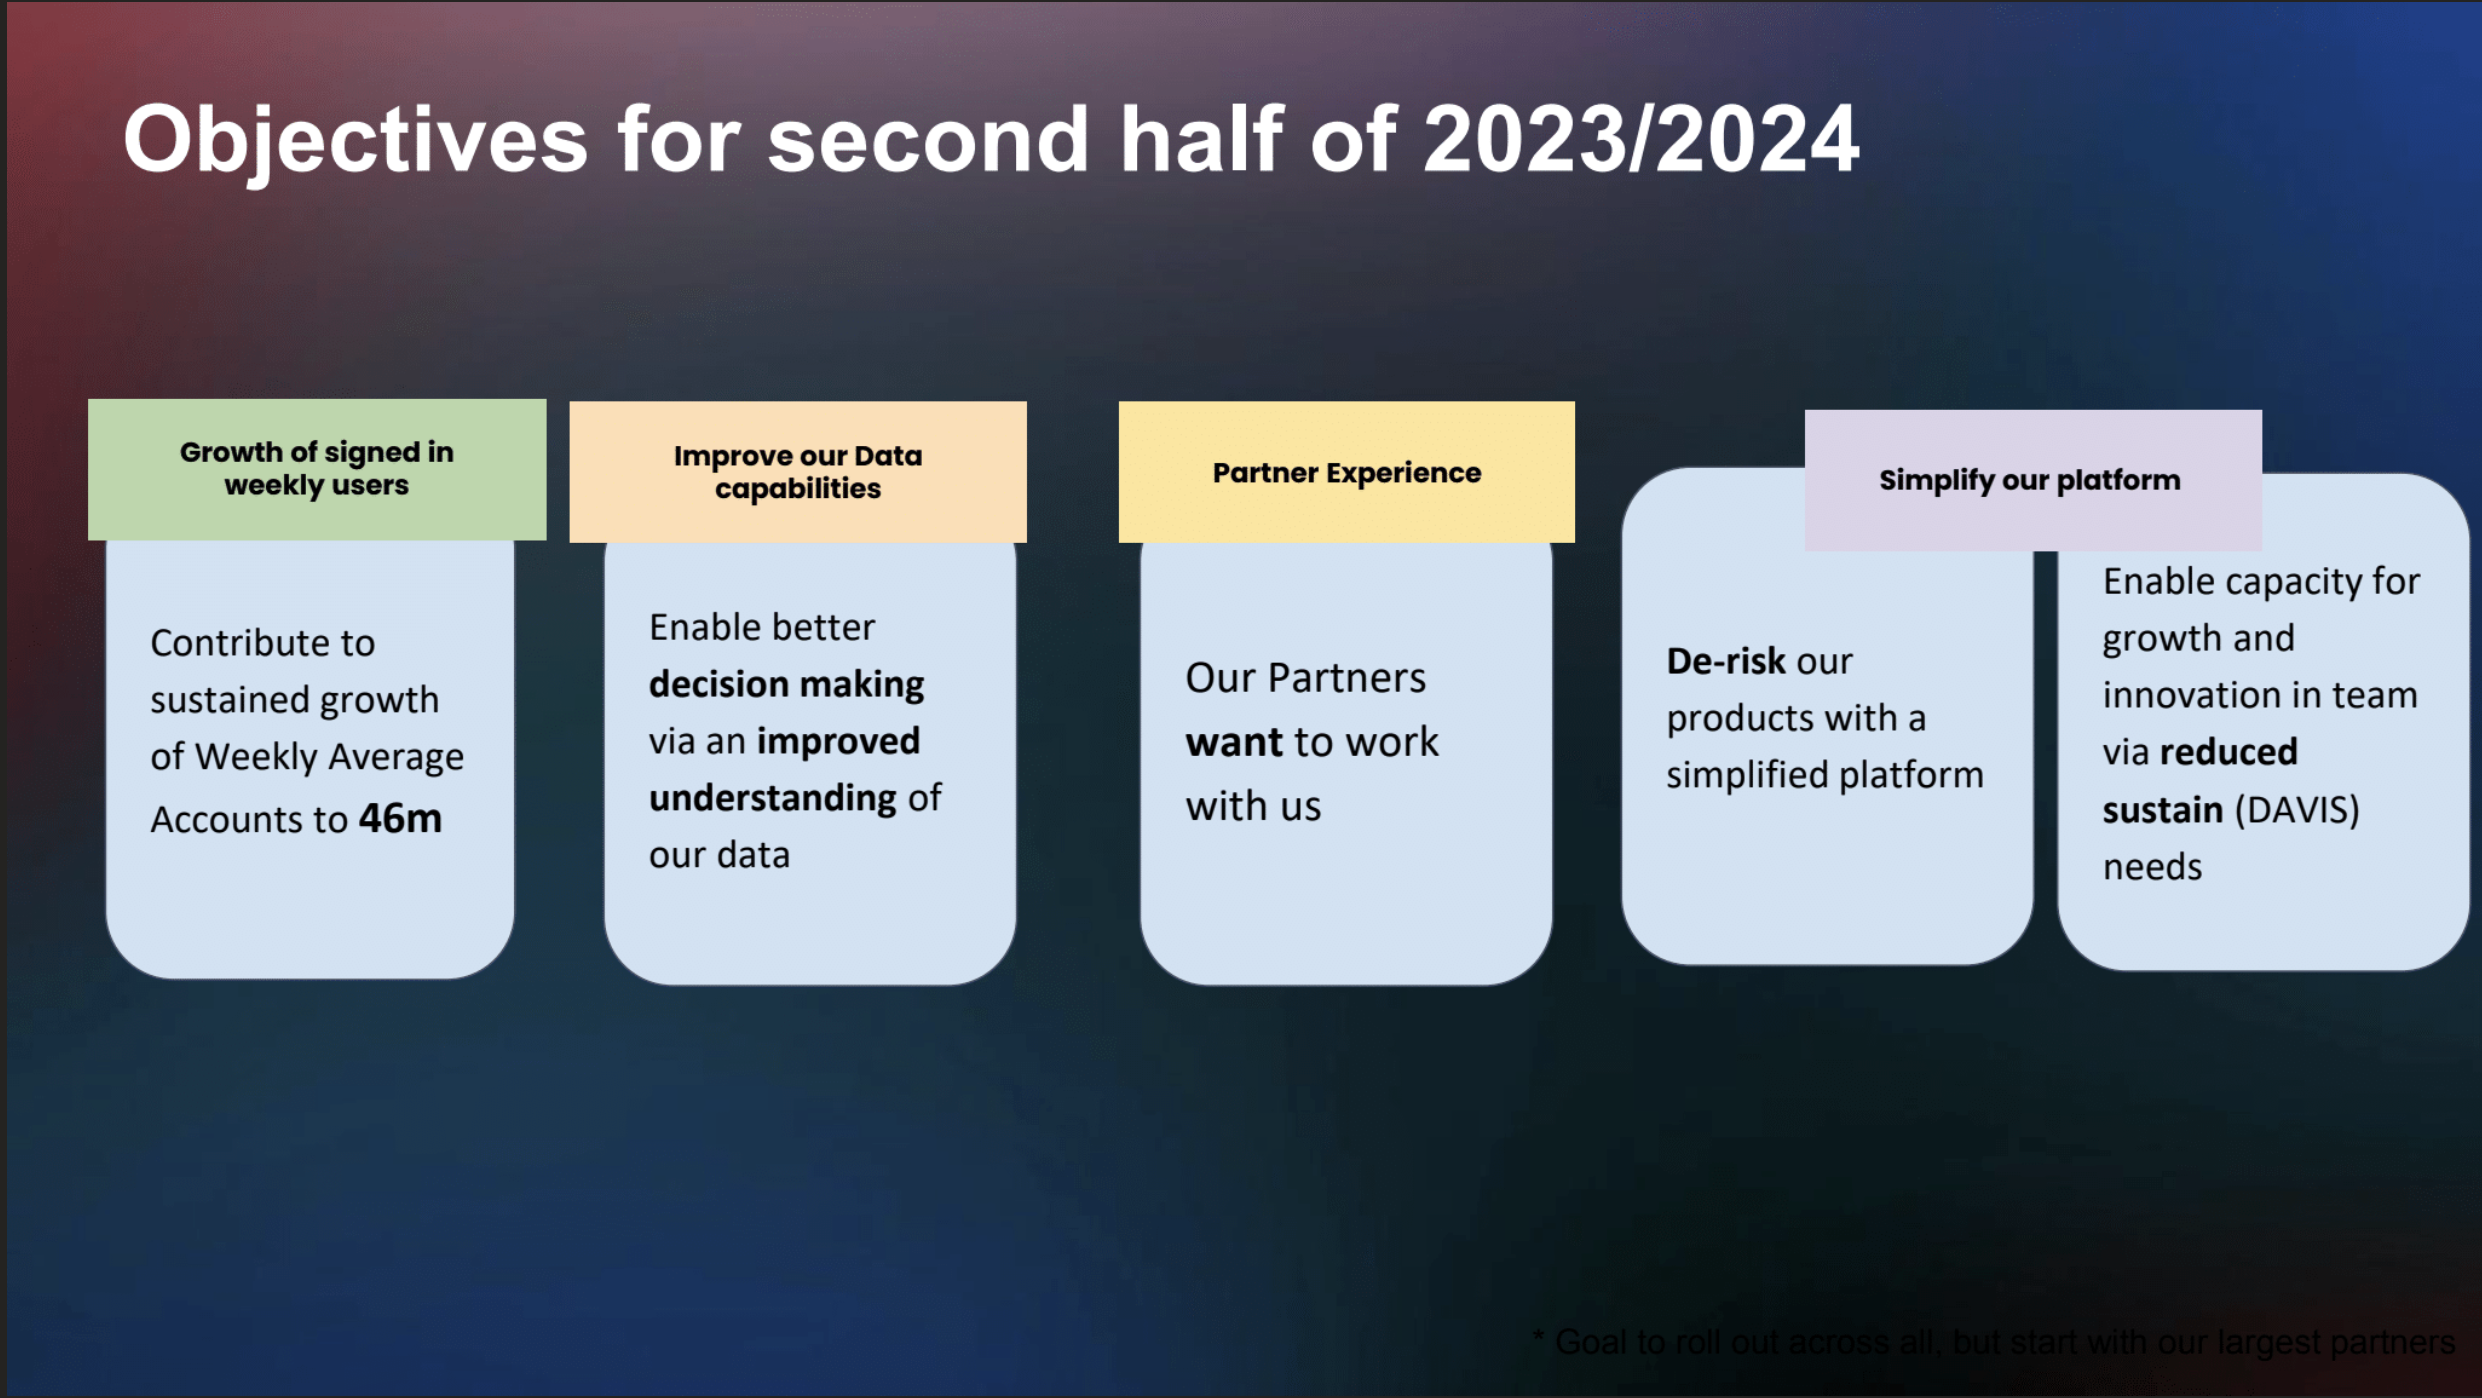
\includegraphics[width=12cm]{assets/appendix/partnershipsObjectives.png}
      \caption{Image taken from a presentation given at a partnerships context setting event (BBC Partnerships, 2023).}
      \label{fig:partnershipsObjectives}
    \end{figure}

  \newpage
  \subsection{Appendix B - Full schedules design including future external notification work}
    \label{sec:AppendixB}
    \begin{figure}[H]
      \centering
      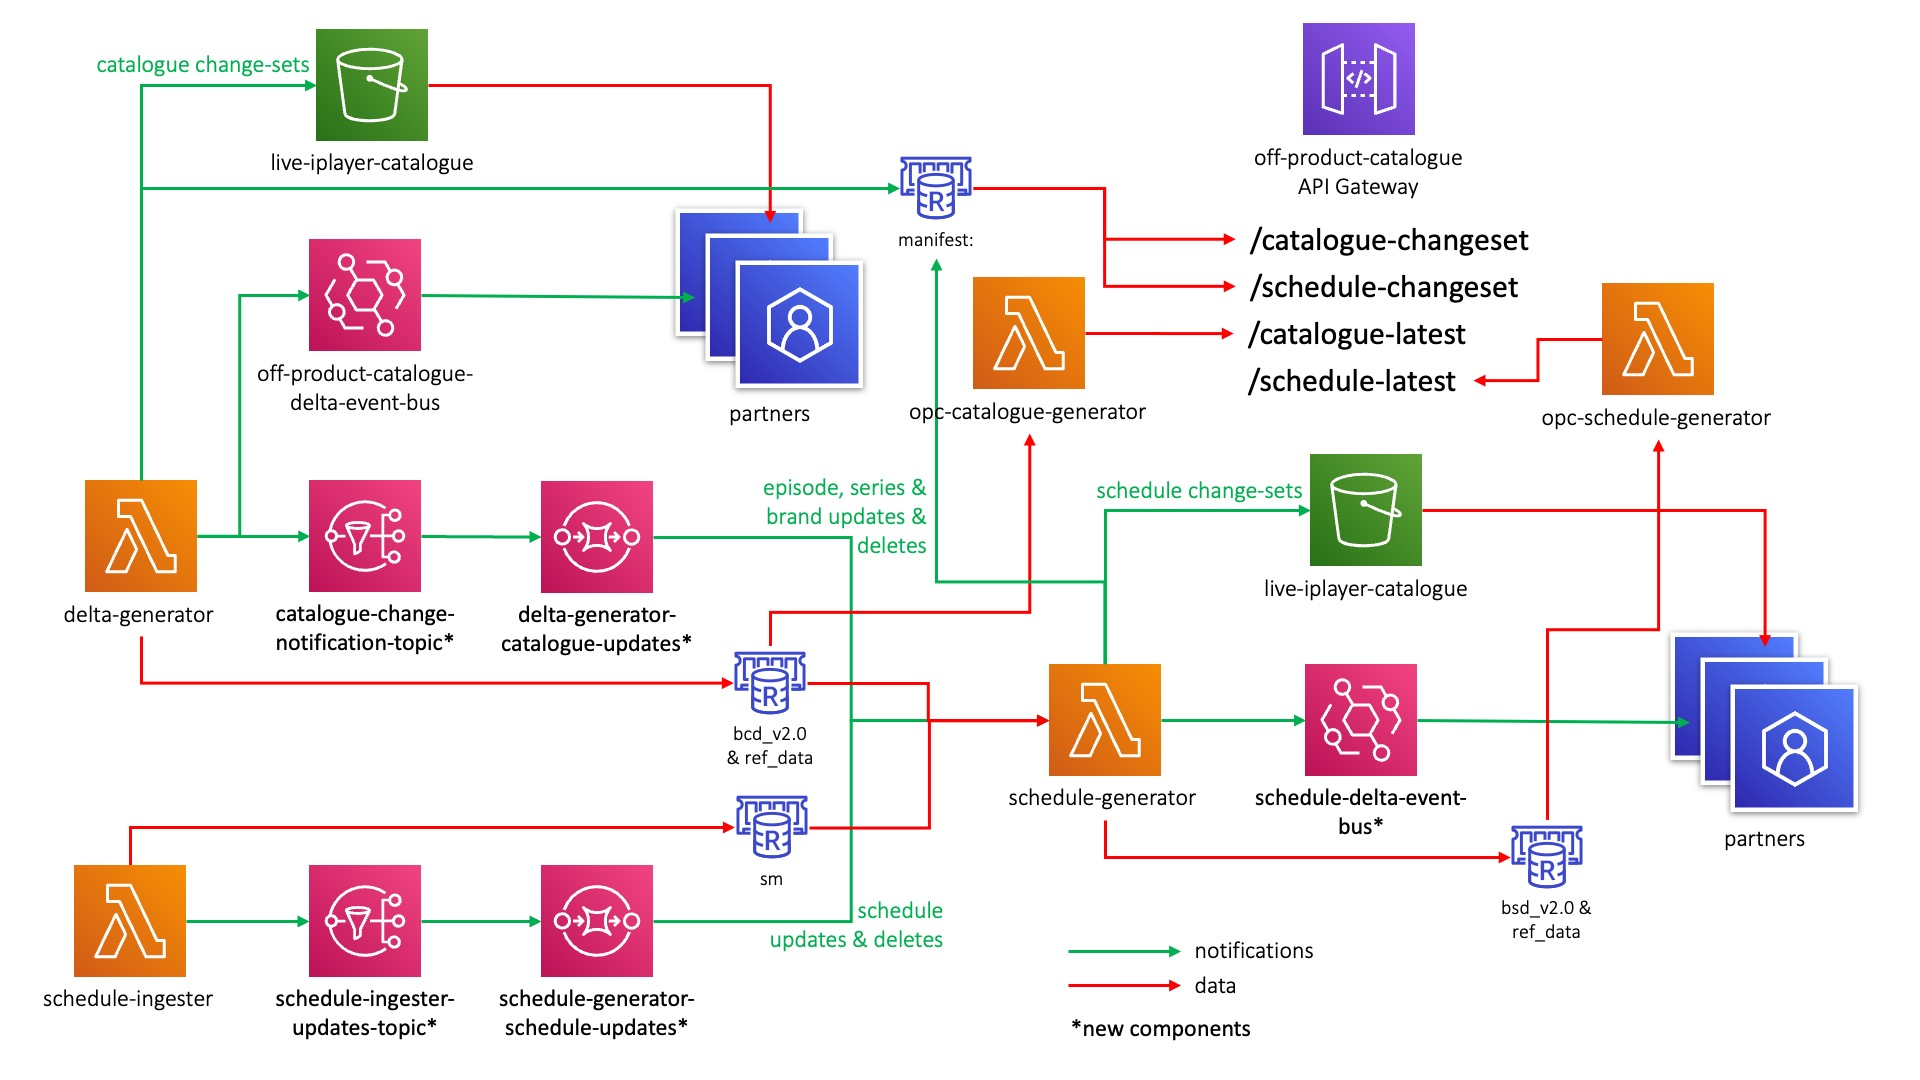
\includegraphics[width=12cm]{assets/appendix/initialDesign.jpg}
      \caption{Full diagram of design for schedules pipeline, including future notifications to partners work (Lloyd, 2023).}
      \label{fig:fullSpikeDesign}
    \end{figure}


  \newpage
  \subsection{Appendix C - Initial flow diagrams for how events would be processed}
    \label{sec:AppendixC}
    \begin{figure}[H]
      \centering
      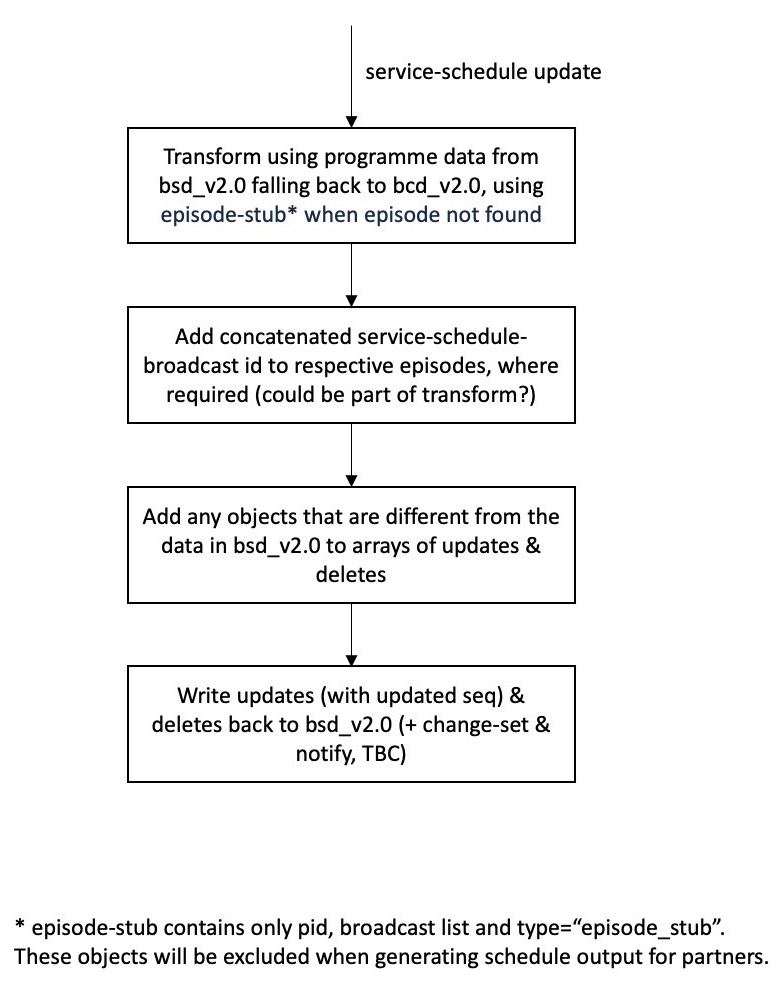
\includegraphics[width=6cm]{assets/initialDesign/scheduleUpdate.jpeg}
      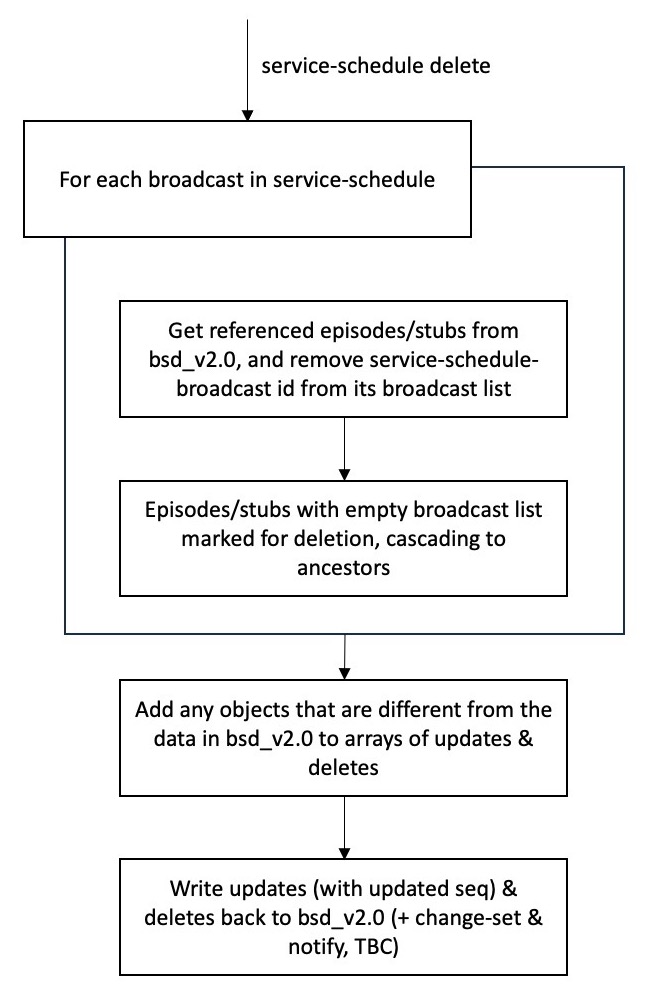
\includegraphics[width=6cm]{assets/initialDesign/scheduleDelete.jpeg}
      \caption{Flow diagrams for schedule events (Lloyd, 2023).}
      \label{fig:initialDesignSchedules}
    \end{figure}


    \begin{figure}[H]
      \centering
      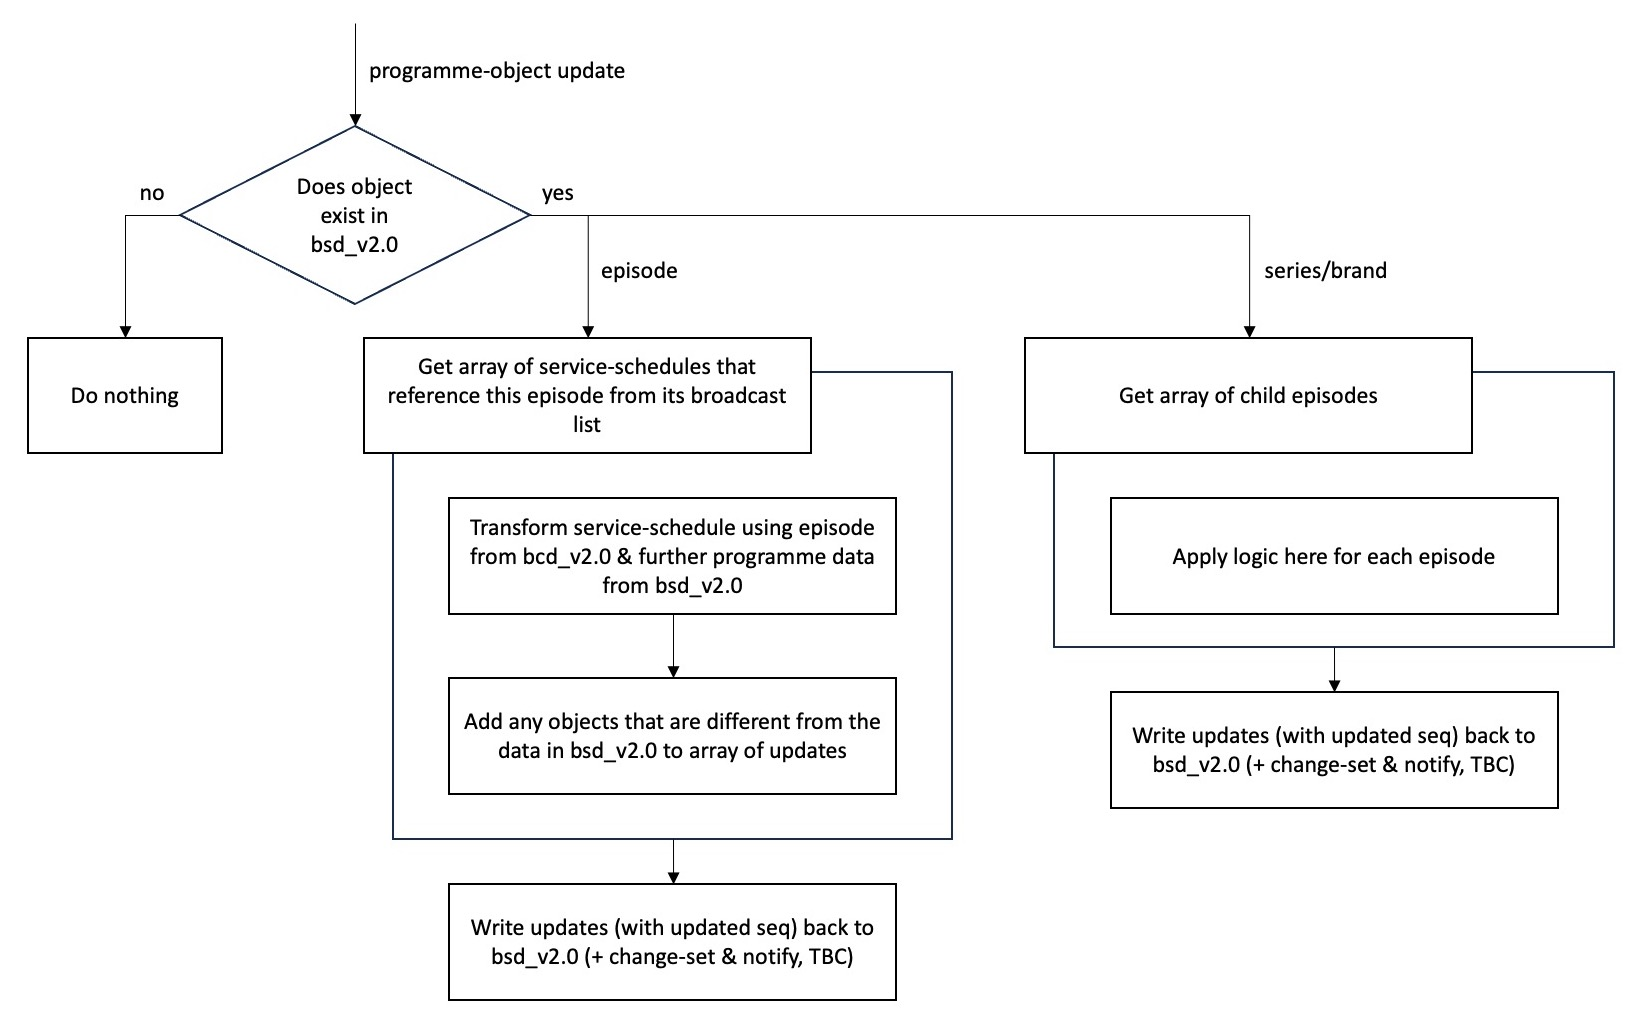
\includegraphics[width=12cm]{assets/initialDesign/programmeUpdate.jpg}
      \caption{Flow diagram for catalogue/programme events (Lloyd, 2023).}
      \label{fig:initialDesignProgrammes}
    \end{figure}

  
  \newpage
  \subsection{Appendix D - Full software spike document}
    \label{sec:AppendixD}
    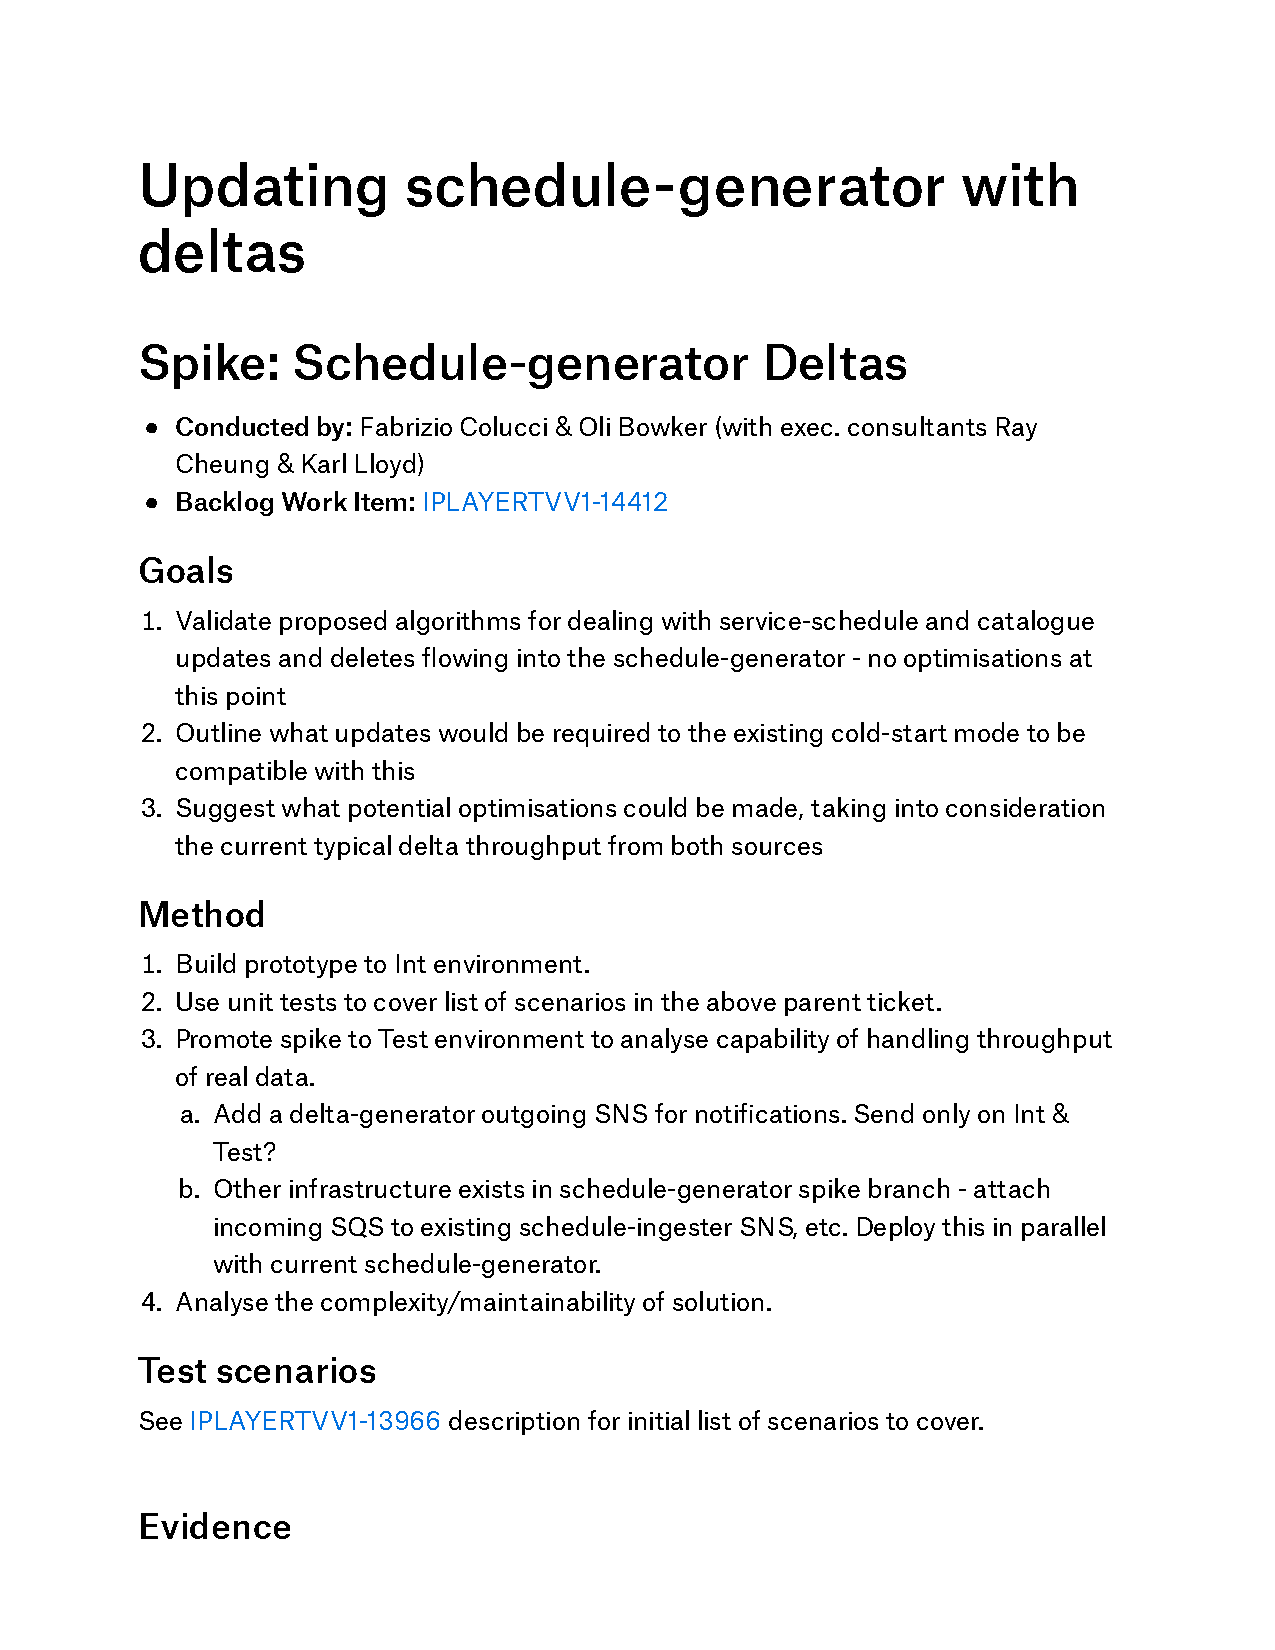
\includepdf[pages=-,scale=.6]{documents/spike.pdf}

  \newpage
  \subsection{Appendix E - Architectural decision for single schedules store}
  \label{sec:AppendixE}

  \subsection*{Architecture Decision Record 022: Single source for schedule data}

  \subsubsection*{Context}
  Schedule documents rely on catalogue data for titling, programme descriptions, subtitling and viewer discretion data. When requesting 
  schedules via the API Gateway the partner also receives episode, series and brand data associated with the schedules requested as part of
  the response. This data can be retrieved from the catalogue redis store but the schedules pipeline is then fully reliant on the catalogue pipeline.
  This reliance of the catalogue pipeline (\emph{{bcd\_v2.0}:}) means that the schedule API gateway is not independent therefore it was requested to make 
  catalogue data more integrated within the schedule redis stores. This ADR describes the decision made to ensure data independence.
  \subsubsection*{Decision}
  Copy over all catalogue data currently relating to schedules into the keyspace \emph{{bsd\_v2.0}:} and \emph{{bsd\_v2.0\_ref\_data}:} respectively on 
  notification events or coldstart. This ensures the API Gateway can retrieve all of its information from one source and keep it's integrity and
  self-consistency. This data should also be removed when no longer referenced by any schedules.

  \subsubsection*{Status}
  Accepted

  \subsubsection*{Consequences}
    \begin{itemize}
      \item Overhead of copying over data existing data.
      \item Added maintenance and code complexity.
      \item Potential synchronisation issue when copying/deleting data across redis stores.
    \end{itemize}


  \newpage
  \subsection{Appendix F - !TODO! List of e2e test scenarios}
    \label{sec:AppendixF}
    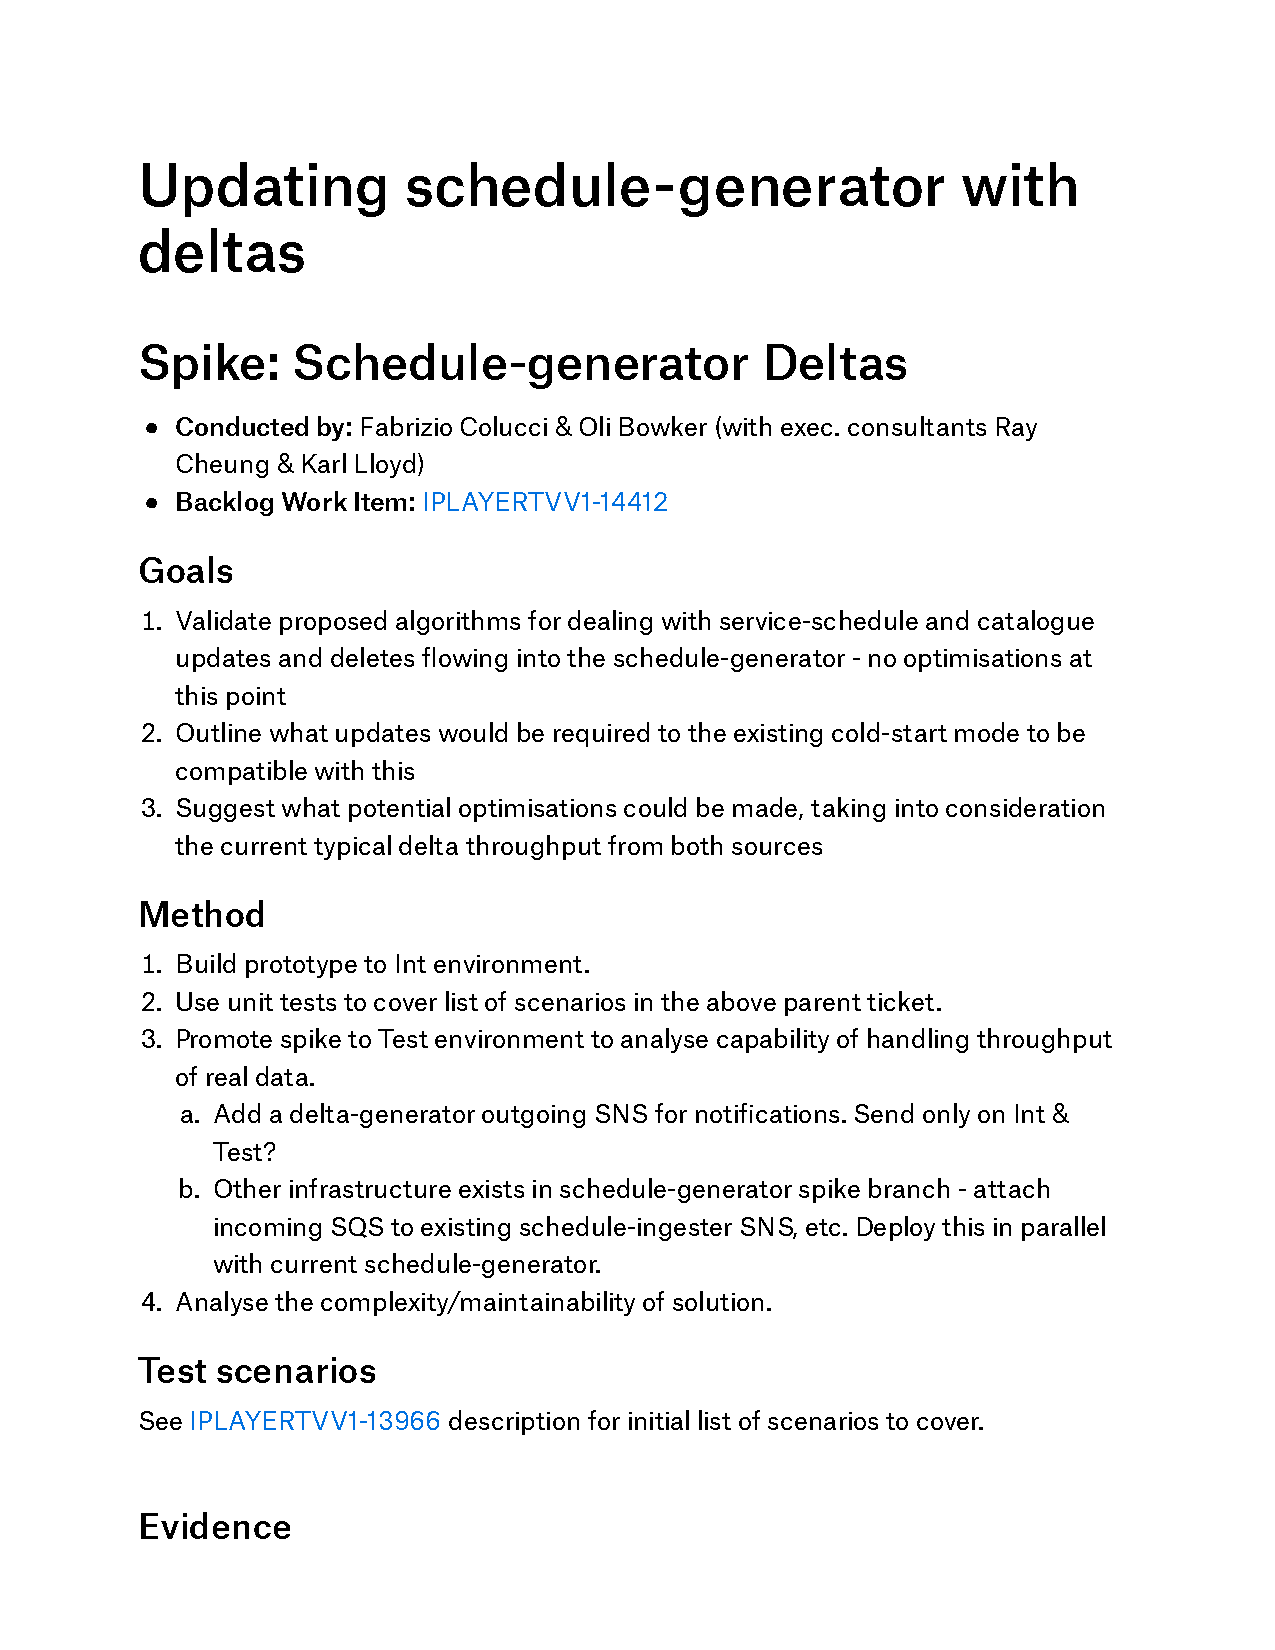
\includepdf[pages=-,scale=.6]{documents/spike.pdf}
  
  \newpage
  \subsection{Appendix !TODO! - Competency Mappings and Links}
    \begin{longtable}{|p{2.5cm}|p{10cm}|p{1.5cm}|}
      \hline
      \textbf{Competency} & \textbf{Description} & \textbf{Page} \\ \hline
      B1                  & Identify, document, review, and design complex IT-enabled business
                            processes that define a set of activities that will accomplish specific
                            organisational goals and that provide a systematic approach to im-
                            proving those processes. & \hyperref[sec:cicd]{Page X} \\ \hline

      P3                  & Professionally present digital-and-technology-solution-specialism plans
                            and solutions in a well- structured business report. & \hyperref[sec:cicd]{Page X} \\ \hline

      P4                  & Demonstrate self-direction and originality in solving problems, and
                            act autonomously in planning and implementing digital-and-technology-
                            solution-specialist tasks at a professional level. & \hyperref[sec:cicd]{Page X} \\ \hline

      P5                  & Be competent at negotiating and closing techniques in a range of
                            interactions and engagements, both with senior internal stakeholders
                            and external stakeholders. & \hyperref[sec:cicd]{Page X} \\ \hline

      SE-S01              & Architect, build, and support leading-edge concurrent-software plat-
                            forms that are performant to industry standards and that deliver
                            responsive solutions with good test coverage. & \hyperref[sec:cicd]{Page X} \\ \hline

      SE-S02              & Drive the technology-decision-making and development process for
                            projects of varying scales, considering current technologies including
                            DevOps and Cloud Computing, and evaluate different technology-
                            design and implementation options, making reasoned proposals and
                            recommendations. & \hyperref[sec:cicd]{Page X} \\ \hline

      SE-S03              & Develop and deliver distributed or semi-complex software solutions
                            that are scalable, and that deliver innovative user experiences and
                            journeys that encompass cross-functional teams, platforms, and technologies. & \hyperref[sec:cicd]{Page X} \\ \hline

      SE-S04              & Update current software products, improving their efficiency and
                            functionality, and build new features to product specifications. 
                          
                          & This project is an upgrade to an existing component and these upgrades will improve the data we provide to partners 
                          bu having our stores as up to date as is possible.  \\ \hline

      SE-S05              & Accomplish planned software-development tasks that deliver the expected
                            features within specified time constraints, security, and quality requirements. & \hyperref[sec:cicd]{Page X} \\ \hline

      SE-S06              & Be accountable for the quality of deliverables from one or more
                            software-development teams (source code quality, automated testing,
                            design quality, documentation, etc.), and following company-
                            standard processes (code reviews, unit testing, source code management, etc.)  & \hyperref[sec:cicd]{Page X} \\ \hline

      SE-K02              & The various inputs, statements of requirements, security considerations
                            and constraints that guide solution architecture and the development
                            of logical and physical systems' designs. & \hyperref[sec:cicd]{Page X} \\ \hline

      SE-K03              & The methodologies designed to help create approaches for organizing
                            the software-engineering process, the activities that need to be
                            undertaken at different stages in the life-cycle, and techniques for
                            managing risks in delivering software solutions. & \hyperref[sec:cicd]{Page X} \\ \hline

      SE-K04              & The approaches used to modularise the internal structure of an
                            application, and to describe the structure and behaviour of applications
                            used in a business, with a focus on how they interact with each other
                            and with business users. & \hyperref[sec:cicd]{Page X} \\ \hline

      SE-K05              & How to design, develop, and deploy software solutions that are secure
                            and effective in delivering the requirements of stakeholders, and
                            the factors that affect the design of a successful code. & \hyperref[sec:cicd]{Page X} \\ \hline

      SE-K06              & The range of metrics which might be used to evaluate a delivered
                            software product. & \hyperref[sec:cicd]{Page X} \\ \hline

      
    \end{longtable}

\end{document}